\chapter{Hardware Characterisation}
\label{chap:hardware}
\chaptoc{}

% ########################################

\newpage
\section{Introduction}
\label{sec:hardware_intro}
\begin{colsection}

In this chapter I detail my work characterising and modelling the GOTO hardware. This work was carried out predominantly in the first year and a half of my PhD, prior to GOTO's commissioning in 2017.
%
\begin{itemize}
    \item In \nref{sec:detectors} I describe and give the results of the detector characterisation tests I ran on the GOTO cameras in the laboratory in Sheffield.
    \item In \nref{sec:throughput} I detail creating a throughput model for the GOTO optical system, in particular examining the Baader filters GOTO uses.
    \item In \nref{sec:photometry} I apply the results of the previous two sections to predict the photometric properties of GOTO images, before comparing them to real observations taken once GOTO was fully operational.
\end{itemize}
%
All work described in this chapter is my own, and has not been published anywhere else.

\end{colsection}

% ########################################

\newpage
\section{Detector properties}
\label{sec:detectors}
\begin{colsection}

% ~~~~~~~~~~~~~~~~~~~~

\begin{colsection}

CCD cameras have a variety of characteristic parameters, including sources of noise. Analysing these under laboratory conditions is important to fully profile them before they are used to take scientific images.

\end{colsection}

% ~~~~~~~~~~~~~~~~~~~~
\subsection{Sources of CCD noise}
\label{sec:noise}
\begin{colsection}

There are many possible sources of noise in images taken with CCD cameras \citep{CCDs}. The most important noise sources for astronomical images are:

\begin{itemize}
    \item \emph{Shot noise} derived from counting photo-electrons from the source object.
    \item \emph{Dark current noise} from thermally generated electrons within the sensor.
    \item \emph{Read-out noise} from the camera electronics.
    \item \emph{Fixed-pattern noise} from different sensitivities between pixels.
    \item \emph{Bias count}, a fixed level of output for each pixel.
\end{itemize}

The shot noise ($\sigma_\text{O}$) arises as photons from the target object arrive at the sensor at different times. The photon arrival time is a Poisson distribution, and if the number of electrons counted is $N$ for large numbers it tends towards a Gaussian distribution with mean $N$ and standard deviation $\sigma_O = \sqrt{N}$. When carrying out on-sky astronomical observations the source noise is typically divided into noise from the target object and noise from the background sky, but that is not relevant in this section.

Dark current noise ($\sigma_\text{D}$) is due to electrons produced by thermal excitations, these are indistinguishable from photo-electrons and will increase with exposure time. As this is also a photon counting measurement it also follows a Poisson distribution, so the noise $\sigma_D = \sqrt{D}$ where $D$ is the dark current per pixel. The dark current depends on temperature, and cooling the cameras will reduce the thermal excitations.

\newpage

Read-out noise ($\sigma_\text{RO}$) depends on the speed data is read out from the CCD.\ The FLI MicroLine cameras read out at a fixed \SI{8}{\mega\hertz}, but other astronomical cameras have variable read-out speeds. As a property of the output electronics the read-out noise is independent of signal or the exposure time used, and therefore it can be represented by a constant value, $\sigma_R = R$, measured in electrons. The MicroLine cameras have two channels with independent readouts, so each will have an independent read-out noise.

Fixed-pattern noise ($\sigma_\text{FP}$) is due to the small differences in size and response between pixels. It it increases linearly with the electron count, including both source and dark electrons (the fixed-pattern noise can be further broken down into the photo response non-uniformity and dark signal non-uniformity, but we will consider it as a single noise source). It can be parametrised as $\sigma_\text{FP} = k_\text{FP}(N+D)$ where $k_\text{FP}$ is a dimensionless constant of proportionality describing the fixed-pattern noise as a percentage of the full-well capacity. Scientific CCD cameras typically have very small non-uniformities between pixels, so $k_\text{FP}$ is usually $<1\%$, but this noise source can dominate when the signal count is high. It can however be removed by flat fielding, so contribution from the fixed-pattern noise is negligible in calibrated astronomical images.

Finally, the bias level is a fixed output of counts from each pixel, and is entirely independent of the input signal. It is therefore the easiest noise source to account for, as once a master bias frame has been constructed it can simply be subtracted from each frame. The MicroLine cameras also include an overscan region (see \aref{sec:chip_layout}), which gives an independent measurement of the bias level for every image.

The noises described above (aside from the bias) are all independent Gaussian random variables, and therefore are added in quadrature to get the total noise per pixel

\begin{equation}
    \begin{split}
        \sigma_\text{Total}^2 & = \sigma_\text{O}^2 +
                                  \sigma_\text{DC}^2 +
                                  \sigma_\text{RO}^2 +
                                  \sigma_\text{FP}^2 \\
                              & = N + D + R^2 + k_\text{FP}^2{(N+D)}^2.
    \end{split}
    \label{eq:noise}
\end{equation}

\end{colsection}

% ~~~~~~~~~~~~~~~~~~~~
\newpage
\subsection{In-lab tests}
\label{sec:camera_tests}
\begin{colsection}

The initial deployment of GOTO was delayed for several months, due to delays on-site at the observatory on La Palma and manufacturing the unit telescopes. The cameras however had already been purchased from FLI, and the delay gave time to test them in the lab in Sheffield. The second set of cameras were also purchased long before the second four unit telescopes were built, these were also bought to Sheffield so the same tests could be repeated.

A list of the nine FLI cameras bought for GOTO is given in \aref{tab:cameras}. Each camera is given a name (Camera 1, Camera 2 etc.) based on the order of their serial numbers. These do not match which GOTO unit telescope they were assigned to, and the cameras on La Palma are sometimes swapped around to allow for repairs.

The first set of four cameras arrived in Warwick in February 2016, and one (Camera 2) was bought to Sheffield in March with a collection of other hardware. The other three were delivered in May and Camera 2 was returned to Warwick, these three were returned in June. The second set cameras were delivered to Warwick in April 2018: four for the next four unit telescopes as well as a spare. The second four cameras (5--8) were brought to Sheffield in May, with Warwick keeping the spare for their own use, these were returned in June.

\begin{table}[t]
    \begin{center}
        \begin{tabular}{c|ccc} %chktex 44
            Name     & Serial number & Set & Tested \\
            \midrule
            Camera 1 & ML0010316     &   1 & May---June 2016  \\
            Camera 2 & ML0330316     &   1 & March---May 2016 \\
            Camera 3 & ML0420516     &   1 & May---June 2016  \\
            Camera 4 & ML0430516     &   1 & May---June 2016  \\
            Camera 5 & ML5644917     &   2 & May---June 2018  \\
            Camera 6 & ML6054917     &   2 & May---June 2018  \\
            Camera 7 & ML6094917     &   2 & May---June 2018  \\
            Camera 8 & ML6304917     &   2 & May---June 2018  \\
            Camera 9 & ML6314917     &   2 & N/A              \\
        \end{tabular}
    \end{center}
    \caption[List of GOTO cameras]{
        A list of the 9 GOTO cameras, with assigned names, serial numbers and dates when the tests were carried out.
    }\label{tab:cameras}
\end{table}

The characterisation tests consisted of taking a series of calibration frames with each camera. Three types of images were needed:

\begin{itemize}
    \item Zero-second dark exposures, to construct bias frames (see \aref{sec:bias}).
    \item Long (30 minute) dark exposures at different temperatures, to measure the dark current (see \aref{sec:dc}).
    \item Flat illuminated frames at different exposure times, to construct photon transfer curves (see \aref{sec:ptc}) and measure linearity (see \aref{sec:lin}).
\end{itemize}

The cameras were tested using two different test setups. \aref{fig:dark_photo} shows the setup for taking dark frames: the cameras are face down and covered. The long dark exposures were taken overnight to as much as possible reduce any excess light reaching the detectors. The flat frames were harder to take. A LCD monitor showing a dark screen was used, with sheets of paper between the camera and the monitor to reduce the illumination. This is shown in \aref{fig:flat_photo}.

The camera manufacturer \glsfirst{fli} and detector manufacturer ON Semiconductor both produce specification sheets advertising expected parameters\footnote{ML50100 available at \url{http://www.flicamera.com/spec_sheets/ML50100.pdf}}\textsuperscript{,}\footnote{KAF-50100 available at \href{http://www.onsemi.com/pub/Collateral/KAF-50100-D.PDF}{\texttt{http://www.onsemi.com/pub/Collateral/KAF-50100-D.pdf}}}, and FLI carried out a limited series of tests on the cameras before selling them. Carrying out our own tests ensures that the cameras meet the specifications, and also allows independent measurements of the key parameters.

\begin{figure}[p]
    \begin{center}
        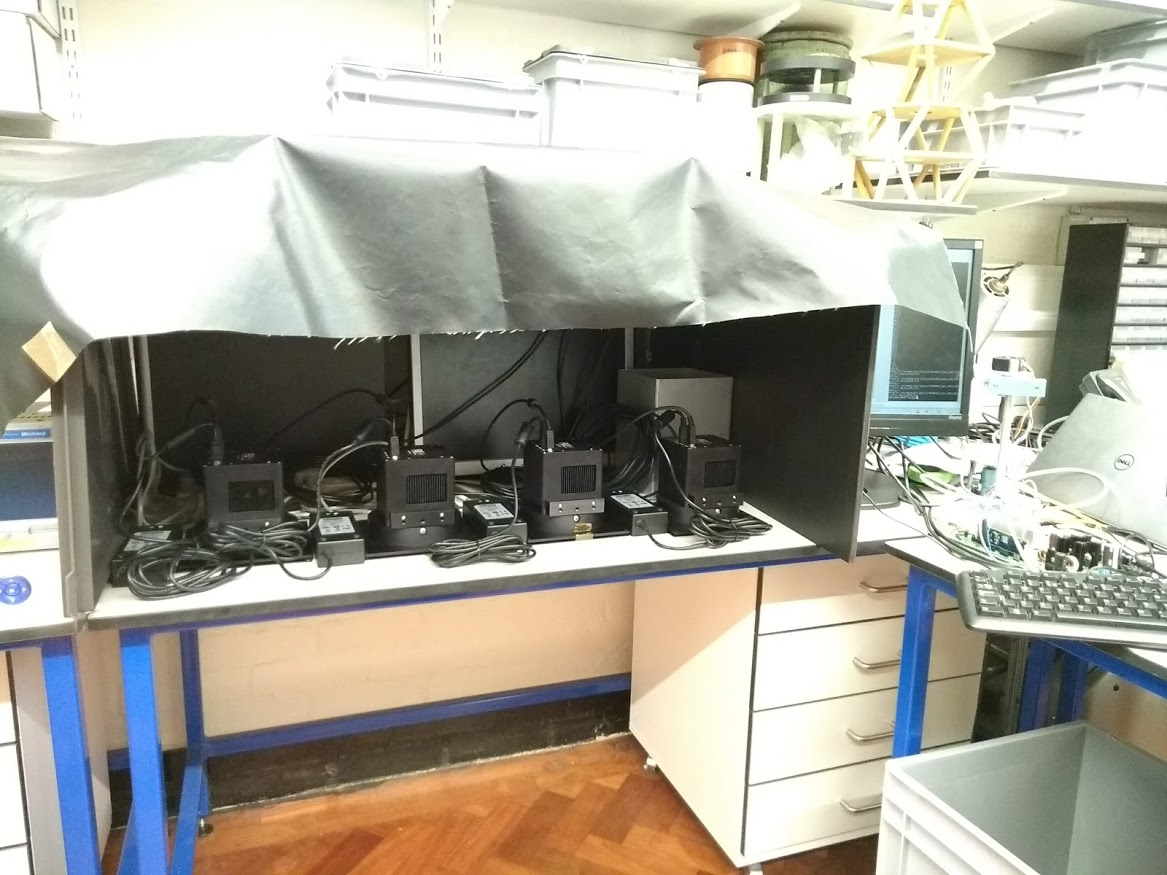
\includegraphics[width=0.75\textwidth]{images/dark_photo.jpg}
    \end{center}
    \caption[The dark frame test setup]{
        A photo of the dark frame test setup in the lab in Sheffield. Dark frames were taken at night with the cover down and ambient light minimised as much as possible.
    }\label{fig:dark_photo}
\end{figure}

\begin{figure}[p]
    \begin{center}
        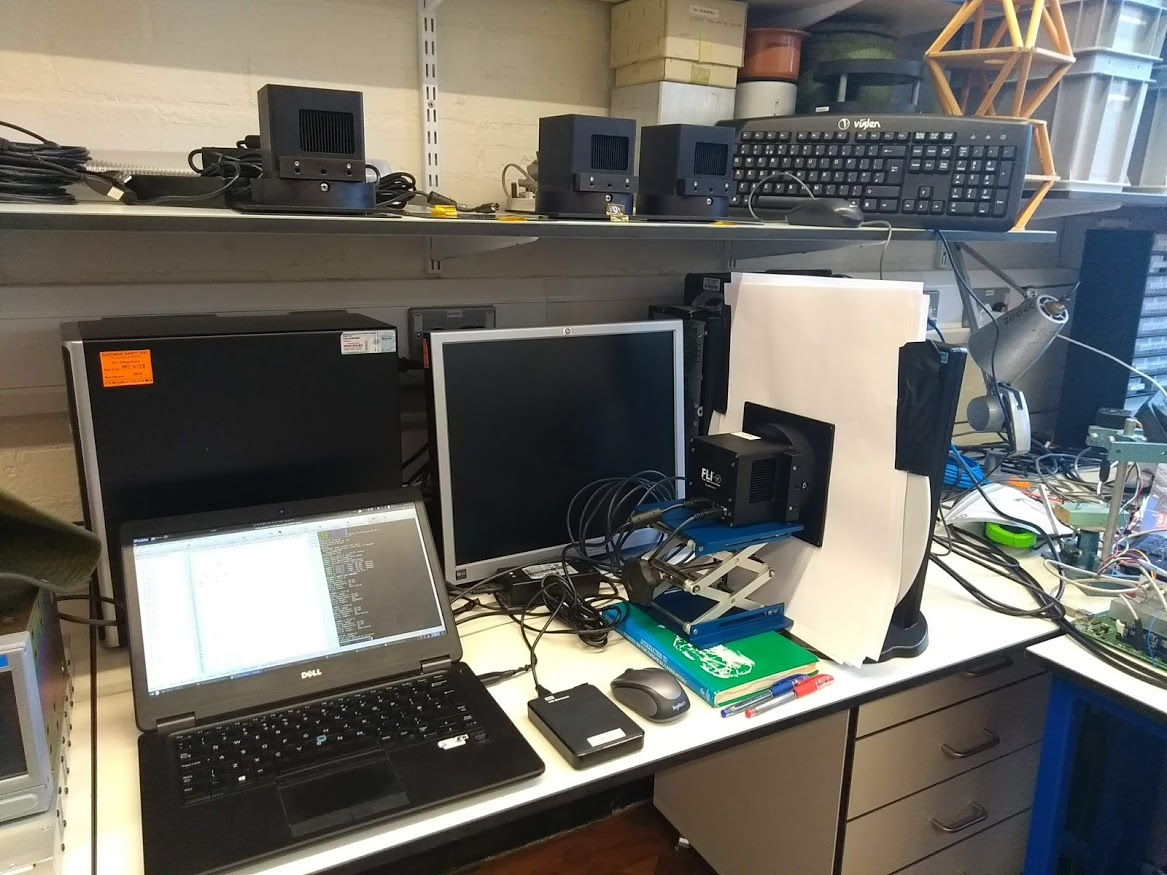
\includegraphics[width=0.75\textwidth]{images/flat_photo.jpg}
    \end{center}
    \caption[The flat frame test setup]{
        A photo of the flat frame test setup. A spare computer monitor was used as a flat screen, with sheets of paper placed in front of the camera to reduce the illumination. The cover shown in \aref{fig:dark_photo} was also placed over the setup.
    }\label{fig:flat_photo}
\end{figure}

\clearpage

\end{colsection}

% ~~~~~~~~~~~~~~~~~~~~
\subsection{Sensor layout}
\label{sec:chip_layout}
\begin{colsection}

The MicroLine ML50100 cameras used by GOTO are contain a KAF-50100 CCD sensor manufactured for FLI by ON Semiconductor\footnote{\url{http://www.onsemi.com/}}. The sensor consists of a 50-megapixel CCD with $\SI{6}{\micro\metre} \times \SI{6}{\micro\metre}$ square pixels. The sensors in the GOTO cameras have two channels each with an independent output, and read out at \SI{8}{\mega\hertz} (variations with four outputs and different readout speeds are also available).

The layout of the sensor is shown in \aref{fig:chip}, adapted from the ON Semiconductor sensor specification sheet. The physical sensor includes $8304 \times 6220$ pixels, while the central region available for data collection has an area of $8176 \times 6132$ pixels. When taking data in full-frame mode the camera outputs an $8304 \times 6220$ array. Surrounding the active area on each edge are 16 \emph{active buffer pixels}, which are light-sensitive but not considered part of the primary region. Around the edge of the active area is a border of light-shielded \emph{dark reference pixels}: 29 dark rows at the start, 26 rows at the end and 28 columns on the sides leading each row. These pixels do not respond to light and therefore can be used as a dark reference. At the beginning and end of each row there is also a test column with 4 blank columns either side, as well as a test row at the end of each frame; these are used to test charge transfer efficiency during the manufacturing process. Finally at the start of each row the register reads out one text pixel, used in the readout process, followed by 10 \emph{dummy pixels} which do not correspond to physical pixels on the sensor. These dummy pixels form an overscan region which can be used to measure the bias level.

A sample frame from Camera 2 is shown in \aref{fig:frame} at high contrast. The extra regions around the frame are visible, including the dark reference and overscan regions.

\begin{figure}[p]
    \begin{center}
        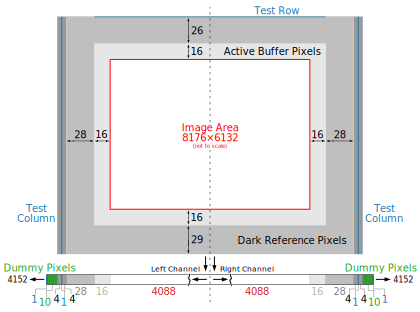
\includegraphics[width=0.85\textwidth]{images/chip}
    \end{center}
    \caption[The layout of the CCD chips in the MicroLine cameras used by GOTO]{
        The layout of the CCD chips in the MicroLine cameras used by GOTO.\@ Note the central image area is not shown to scale.
    }\label{fig:chip}
\end{figure}

\begin{figure}[p]
    \begin{center}
        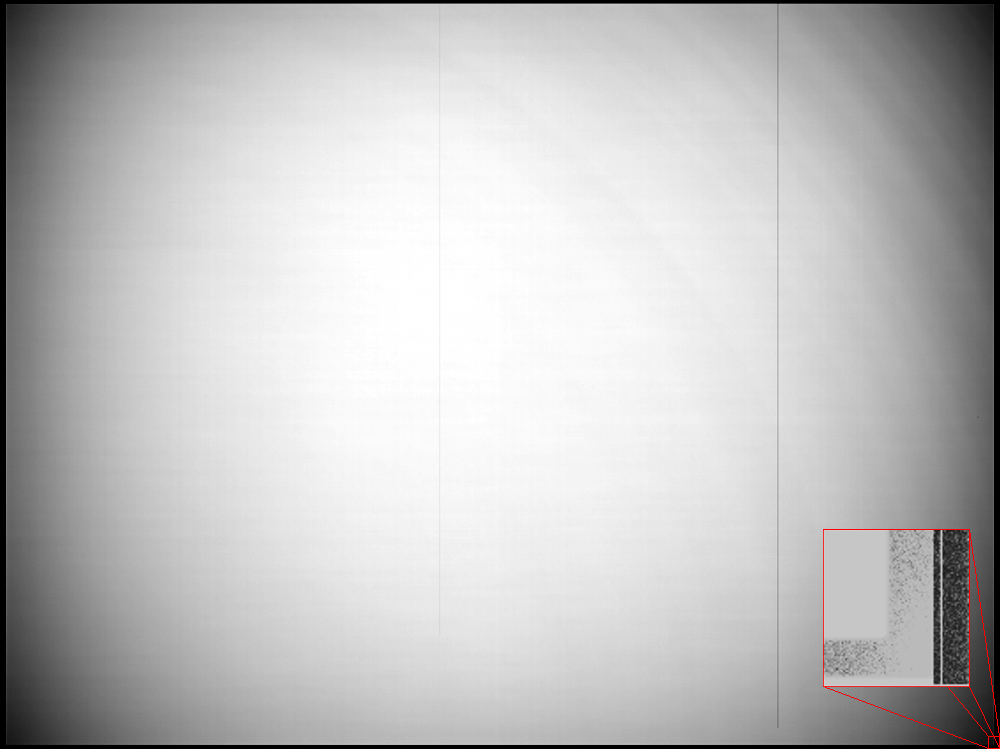
\includegraphics[width=0.7\textwidth]{images/sample.png}
    \end{center}
    \caption[A sample bright frame from one of the MicroLine cameras]{
        A sample bright frame from one of the MicroLine cameras. The highlighted area in the corner shows some of the features described in \aref{fig:chip}.
    }\label{fig:frame}
\end{figure}

\clearpage

\end{colsection}

% ~~~~~~~~~~~~~~~~~~~~
\newpage
\subsection{Bias}
\label{sec:bias}
\begin{colsection}

The bias level is a fixed offset in counts for each pixel. Setting a reasonable bias level in a CCD is important in order to ensure counts are never recorded as negative due to random noise. In general the bias level of each pixel is considered a fixed value, although it can change over time due to degradation of the pixel electronics. Bias should therefore still be measured regularly, as any change might indicate a problem with the detector.

Pixel bias levels can be measured by taking a dark, zero-second exposure time image. This image will not include any electrons from a source, so the shot noise is zero, and as the dark current is proportional to the exposure time this will also be minimised. The image will however still include random read-out noise, so to account for this multiple images are taken and then averaged to produce a master bias frame.

For each of the eight cameras 50 bias images were taken, these were combined to form a master bias frame by taking the median value in each pixel (to account for superfluous counts due to cosmic rays). The mean count in a 2000$\times$2000 pixel region in the centre of each of the two camera channels was measured, using a one-sigma clip to exclude any defect pixels (see \aref{sec:defects}). These values are given in \aref{tab:bias}.

The measured biases are all around the same level, 970--1010 counts, as would be expected. They also have a uniform standard deviation of approximately 0.3--0.4\% of the signal, which will come from the fixed-pattern noise (see \aref{sec:ptc}).

\begin{table}[t]
    \begin{center}
        \begin{tabular}{c|rr} %chktex 44
             & \multicolumn{2}{c}{Bias} \\
             & \multicolumn{2}{c}{(ADU)} \\
             & \multicolumn{1}{c}{L} & \multicolumn{1}{c}{R} \\
            \midrule
            Camera 1 & $971\pm4$ & $969\pm4$ \\
            Camera 2 & $989\pm3$ & $983\pm3$ \\
            Camera 3 & $1004\pm3$ & $991\pm3$ \\
            Camera 4 & $974\pm3$ & $1008\pm4$ \\
        \end{tabular}
        \hspace{0.5cm}
        \begin{tabular}{c|rr} %chktex 44
             & \multicolumn{2}{c}{Bias} \\
             & \multicolumn{2}{c}{(ADU)} \\
             & \multicolumn{1}{c}{L} & \multicolumn{1}{c}{R} \\
            \midrule
            Camera 5 & $994\pm3$ & $986\pm3$ \\
            Camera 6 & $984\pm3$ & $991\pm3$ \\
            Camera 7 & $992\pm3$ & $981\pm3$ \\
            Camera 8 & $1008\pm3$ & $1012\pm3$ \\
        \end{tabular}
    \end{center}
    \caption[Bias values]{
        Bias values for each camera.
    }\label{tab:bias}
\end{table}

\end{colsection}

% ~~~~~~~~~~~~~~~~~~~~
\newpage
\subsection{Gain, read-out noise and fixed-pattern noise}
\label{sec:ptc}
\begin{colsection}

The gain, read-out and fixed-pattern noise of a CCD camera can be measured using the \gls{ptc} method \citep{CCDs, PTC}. To construct a photon transfer curve a series of bright exposures of a flat light source were taken with varying exposure times. For these images the dark current noise is negligible, so once the images has the bias level subtracted the total number of electrons in each pixel, $N_\text{Total}$, will include a number of photo-electrons from the source $N$ plus extra electrons from the readout electronics $R$:

\begin{equation}
    N_\text{Total} = N + R.
    \label{eq:total_count}
\end{equation}

The noise per pixel, excluding dark current, is given by \aref{eq:noise} as

\begin{equation}
    \begin{split}
        \sigma_\text{Total}^2 & = N + R^2 + k_\text{FP}^2 N^2 \\
                              & = N_\text{Total} - R + R^2 + k_\text{FP}^2{(N_\text{Total} - R)}^2.
    \end{split}
    \label{eq:ptc_noise1}
\end{equation}

The counts and total noise here are all in electrons (\elec), however the output of the camera analog-to-digital converter is a digital signal, $S$, measured in \gls{adu}. This signal is linearly related to the actual number of electrons detected $N_\text{Total}$ through the gain $g$, in \elec/ADU, as

\begin{equation}
    N_\text{Total} = g S.
    \label{eq:gain}
\end{equation}

The gain is an important parameter of a CCD detector, and can be set to best utilise the dynamic range of the detector. The KAF-50100 detectors have a specification full well capacity of 40,300 electrons before they saturate, and the cameras have a 16-bit readout (meaning the signal from each pixel can vary from 0 to 65535 ($2^{16}$) ADU). Therefore if the gain was set to $1$ \elec/ADU a saturated pixel would produce a signal of 40300 ADU, which is only using two-thirds of the dynamic range. The ideal gain to utilise the full well capacity for these cameras would therefore be $0.62$ \elec/ADU.\@ However, a high gain introduces a quantisation error due to the random electrons produced by the read-out noise. Setting the gain therefore is a balance between these two effects.

Since \aref{eq:gain} shows the signal $S$ is directly proportional to the number of electrons $N$, their errors are also directly proportional with the same constant. Therefore the noise in the signal, $\sigma_S$, is related to the noise in the total electron count as

\begin{equation}
    \sigma_\text{Total} = g \sigma_S.
    \label{eq:noise_gain}
\end{equation}

Converting the total electron count and noise in \aref{eq:ptc_noise1} into ADU results in

\begin{equation}
    g^2\sigma_S^2 = gS - R + R^2 + k_\text{FP}^2 {(gS - R)}^2,
    \label{eq:ptc_noise2}
\end{equation}

and rearranging this gives the final photon transfer curve equation

\begin{equation}
    \sigma_S^2 = \frac{R^2(1-k_\text{FP}^2) - R}{g^2} + \frac{1}{g}S + k_\text{FP}^2 S^2.
    \label{eq:ptc}
\end{equation}

This is a quadratic equation in $S$ which relates the measured total signal $S$ to the variance in the signal $\sigma_S^2$, where $S$ and $\sigma_S$ are in ADU, read-out noise $R$ is still in \elec, gain $g$ is in \elec/ADU and the fixed-pattern noise parameter $k_\text{FP}$ is dimensionless. Since $k_\text{FP}$ is expected to be a very small fraction, typically less than 1\%, the $(1-k_\text{FP}^2)$ factor is often ignored. As well the constant is often further simplified to just $R^2/g^2$, which could be considered as $R_S^2$ where $R_S$ is measured in ADU.\@ For this test the full equation was used when fitting to the data.

A photon transfer curve is a log-log plot of a signal value against the noise in the signal, here represented by $S$ and standard deviation $\sigma_S$ (the square root of the variance). By fitting \aref{eq:ptc} to this plot values for the gain, read-out noise and fixed-pattern noise can be determined. The key features of a photon transfer curve are common for all CCDs, and are shown in cartoon form in \aref{fig:ptc_cartoon}.

\begin{figure}[t]
    \begin{center}
        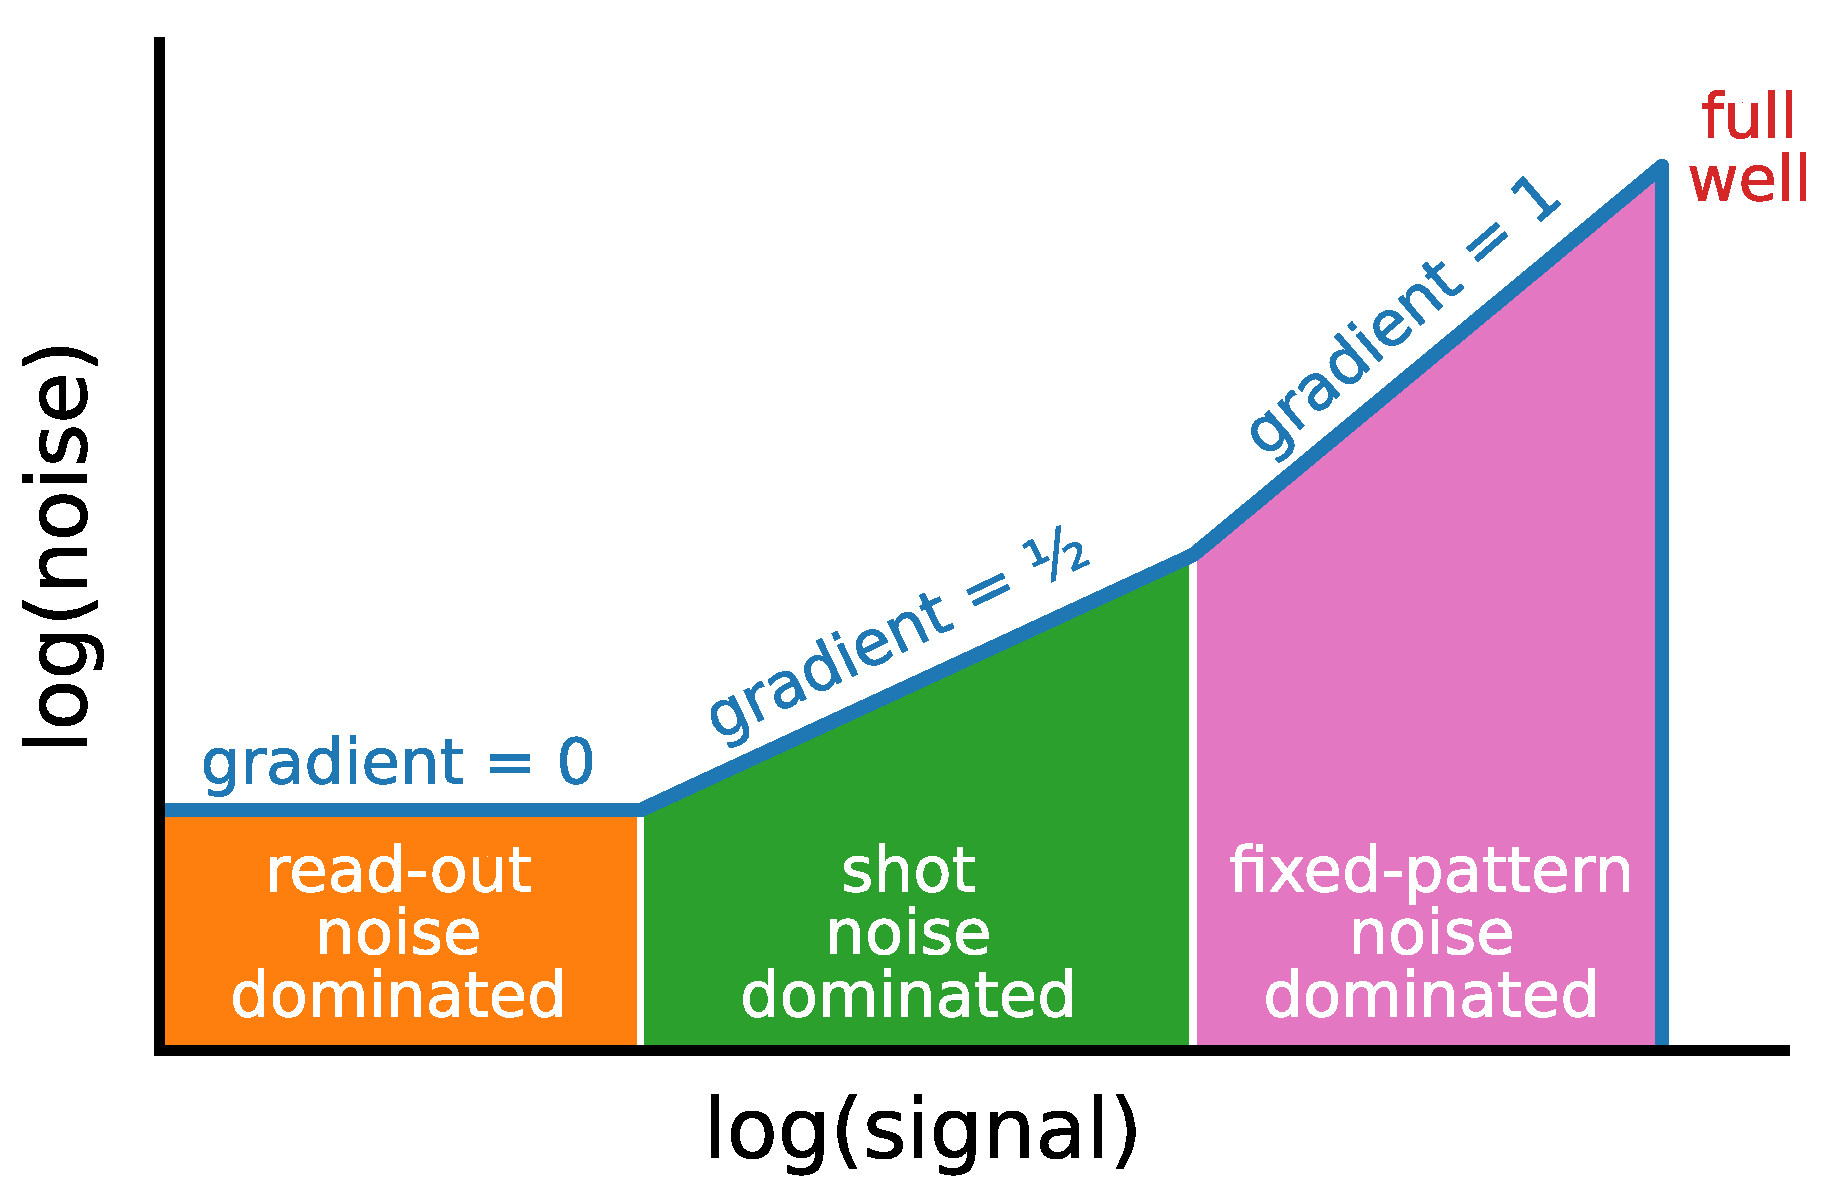
\includegraphics[width=0.75\textwidth]{images/ptc.pdf}
    \end{center}
    \caption[Key features of the photon transfer curve]{
        The key features of a photon transfer curve, adapted from Figure 2.2 of \citet{CCDs}.
    }\label{fig:ptc_cartoon}
\end{figure}

There are three visible noise regimes in the photon transfer curve. The first is when the signal is zero. For small $S$ in \aref{eq:ptc} the noise is constant, and as there is no signal the overall noise is limited by the detector noise. This will include both the read-out noise and the dark current, but as these are very short exposure times (less than 1 second) the dark current is completely negligible and the read-out noise dominates. At higher signals the noise is dominated by the shot noise. As this is proportional to the square root of the signal this region has a gradient of 1/2 when plotted on the log-log axis, and when $\sigma_S$ is zero the signal will equal the gain (i.e.\ the value of the gain is where the linear fit crosses the x-axis). As the signal increases further the fixed-pattern noise begins to dominate over the shot noise, as it is proportional to the signal this produces a gradient of 1 in the \gls{ptc}. Finally the pixel will reach its full well value and saturate, so the noise drops to zero.

As it is impossible to know the exact number of incoming photons on each pixel, it is not possible to determine the signal and noise values for a given pixel. Instead the PTC is constructed by selecting a region of pixels and plotting the mean signal value against the standard deviation. Repeated for several regions across the image this gives a reasonable approximation of the average noise in each pixel.

\begin{table}[t]
    \begin{center}
        \begin{tabular}{l|cc|cc|cc} %chktex 44
             &
            \multicolumn{2}{c|}{Gain} &
            \multicolumn{2}{c|}{RO noise} &
            \multicolumn{2}{c}{FP noise} \\
            &
            \multicolumn{2}{c|}{(\elec/ADU)} &
            \multicolumn{2}{c|}{(\elec)} &
            \multicolumn{2}{c}{(\%)} \\
             & L & R & L & R & L & R \\
            \midrule
            Camera 1 & 0.53 & 0.53 & 12.9 & 12.6 & 0.46 & 0.45 \\
            Camera 2 & 0.53 & 0.53 & 12.4 & 12.2 & 0.44 & 0.46 \\
            Camera 3 & 0.57 & 0.57 & 13.1 & 12.3 & 0.45 & 0.42 \\
            Camera 4 & 0.57 & 0.58 & 14.0 & 14.5 & 0.41 & 0.43 \\
            Camera 5 & 0.62 & 0.63 & 12.8 & 13.3 & 0.40 & 0.40 \\
            Camera 6 & 0.63 & 0.62 & 12.4 & 13.1 & 0.40 & 0.40 \\
            Camera 7 & 0.62 & 0.62 & 13.6 & 13.1 & 0.41 & 0.39 \\
            Camera 8 & 0.62 & 0.62 & 14.8 & 12.8 & 0.41 & 0.39 \\
        \end{tabular}
    \end{center}
    \caption[Gain, read-out noise and fixed-pattern noise values]{
        Gain, read-out noise and fixed-pattern noise values found by fitting photon transfer curves for each camera.
    }\label{tab:ptc}
\end{table}

\glspl{ptc} were constructed for all eight cameras, by taking flat images of varying exposure times. Twelve 50$\times$50 pixel regions were selected across the field, and the mean and standard deviation of the pixel values were plotted to form the \gls{ptc}. These are shown in \aref{fig:ptcs}. The curves were fitted to \aref{eq:ptc}, and the resulting values for the gain ($g$), read-out noise ($R$) and fixed-pattern noise ($k_\text{FP}$) are given in \aref{tab:ptc}.

As expected, the gain values are all around 0.6 \elec/ADU, and would have been set as such to maximise the dynamic range. There is a clear difference in gain levels between the first set of cameras (1--4) and the second set (5--8), which is most likely due to changes made by FLI over the two years between their manufacture.

The read-out noise values match the FLI specifications which advertises a typical system noise of 12 \elec{} when reading out at \SI{8}{\mega\hertz}. The two channels on each camera are independent and therefore there is no correlation in read-out noise, unlike the gain which is always approximately the same in each amplifier.

Finally, as expected the fixed-pattern noise is a low fraction of the signal. It notably decreases from $\sim$0.45\% to $\sim$0.40\%; if this is related to improved chip manufacturing this may be related to the change in gain in the later cameras. However, this test only includes a small sample of the 50 million pixels on each chip and so may not be a perfect measure of the overall photo response non-uniformity. The values for the fixed-pattern noise also match the standard deviations measured in the master biases in \aref{sec:bias}.

\begin{figure}[p]
    \begin{center}
        \begin{minipage}[t]{0.49\textwidth}\vspace{10pt}
            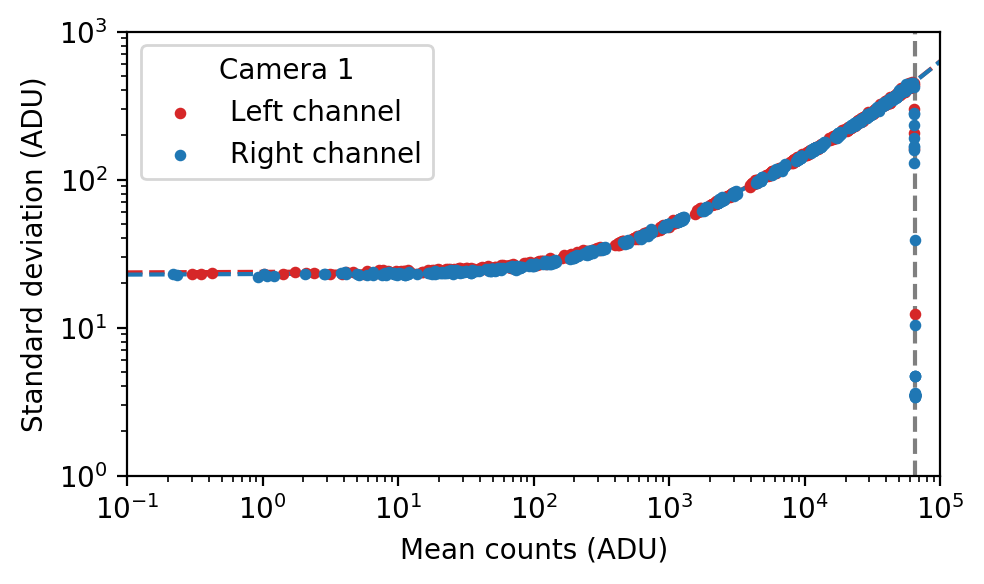
\includegraphics[width=\linewidth]{images/detectors/ptc_1.png}
        \end{minipage}
        \begin{minipage}[t]{0.49\textwidth}\vspace{10pt}
            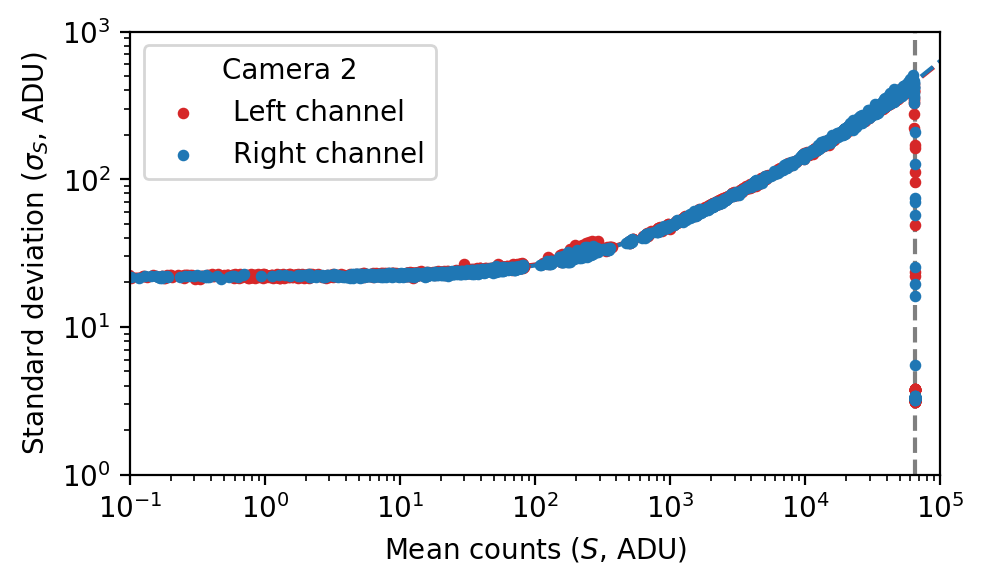
\includegraphics[width=\linewidth]{images/detectors/ptc_2.png}
        \end{minipage}

        \begin{minipage}[t]{0.49\textwidth}\vspace{10pt}
            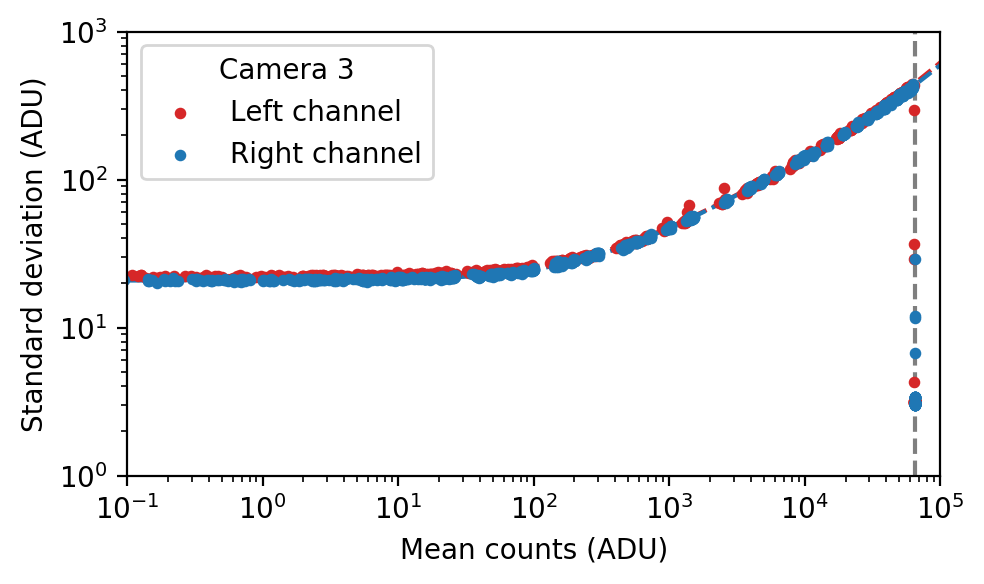
\includegraphics[width=\linewidth]{images/detectors/ptc_3.png}
        \end{minipage}
        \begin{minipage}[t]{0.49\textwidth}\vspace{10pt}
            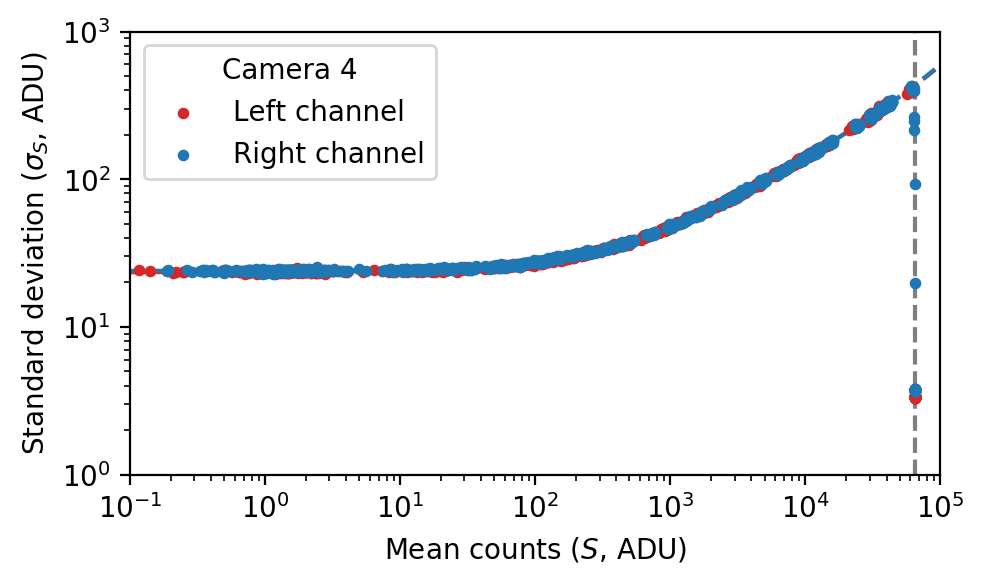
\includegraphics[width=\linewidth]{images/detectors/ptc_4.png}
        \end{minipage}

        \begin{minipage}[t]{0.49\textwidth}\vspace{10pt}
            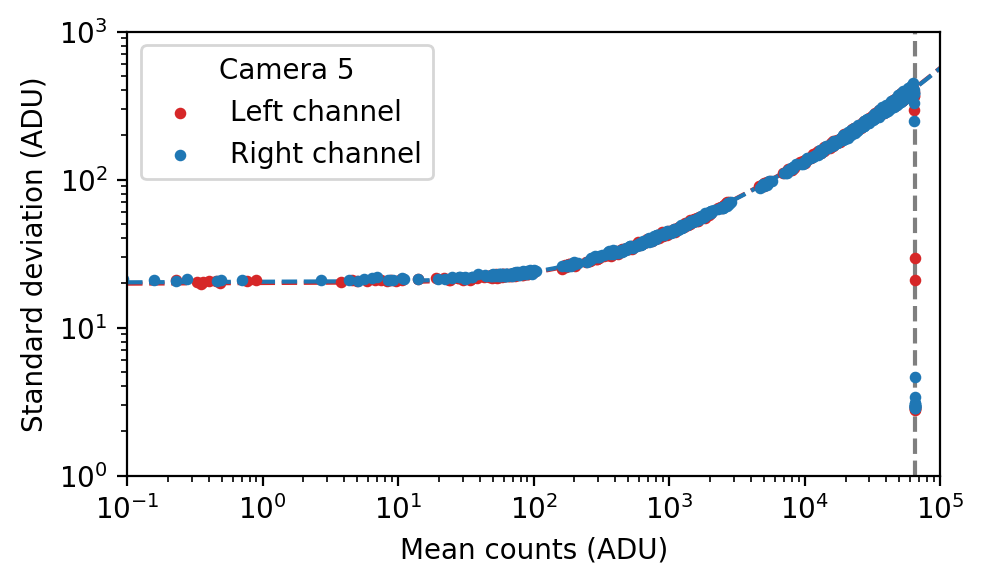
\includegraphics[width=\linewidth]{images/detectors/ptc_5.png}
        \end{minipage}
        \begin{minipage}[t]{0.49\textwidth}\vspace{10pt}
            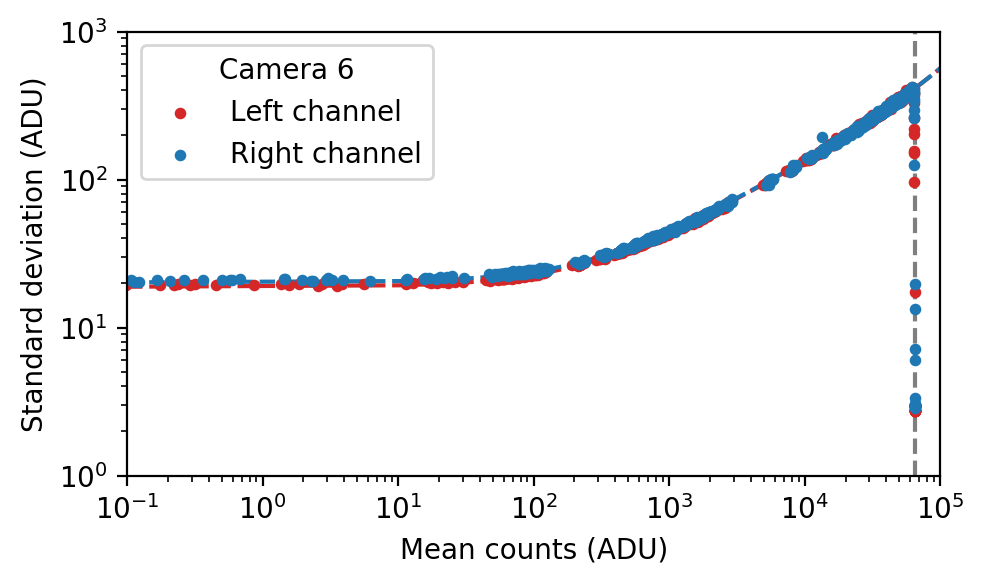
\includegraphics[width=\linewidth]{images/detectors/ptc_6.png}
        \end{minipage}

        \begin{minipage}[t]{0.49\textwidth}\vspace{10pt}
            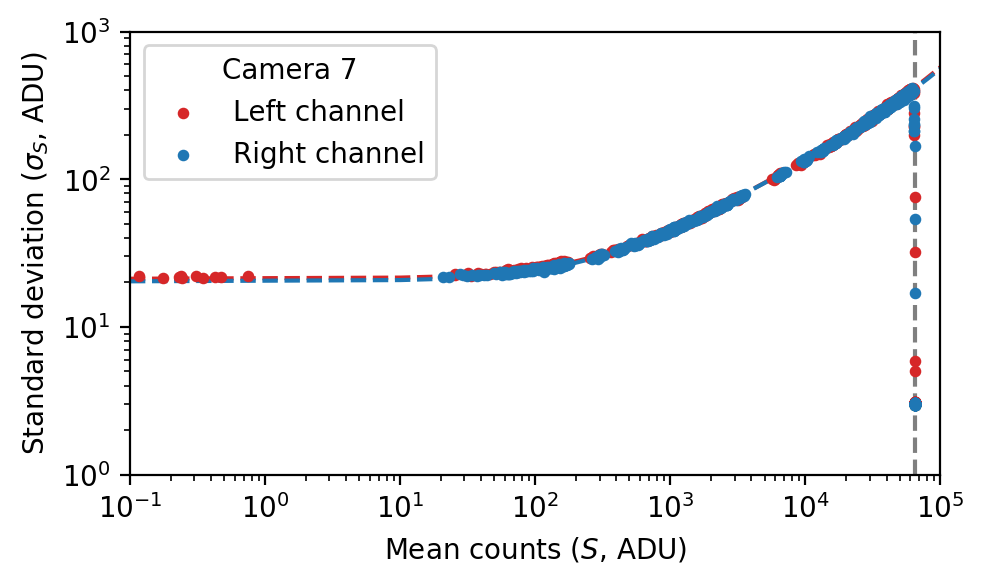
\includegraphics[width=\linewidth]{images/detectors/ptc_7.png}
        \end{minipage}
        \begin{minipage}[t]{0.49\textwidth}\vspace{10pt}
            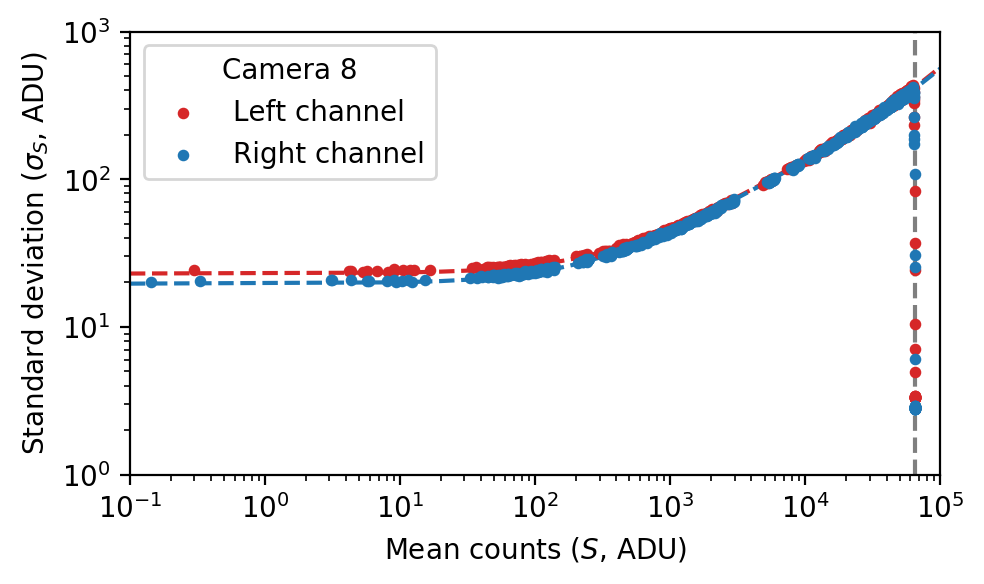
\includegraphics[width=\linewidth]{images/detectors/ptc_8.png}
        \end{minipage}
    \end{center}
    \caption[Photon transfer curve plots]{
        Photon transfer curve plots for each camera.
    }\label{fig:ptcs}
\end{figure}

\clearpage

\end{colsection}

% ~~~~~~~~~~~~~~~~~~~~
\newpage
\subsection{Dark current}
\label{sec:dc}
\begin{colsection}

Dark current is another source of noise in a CCD, produced by thermally excited electrons \citep{dark_current}. The dark current noise is therefore independent of the incoming signal or the exposure time, but increases as a function of temperature, $T$. Specifically the dark current increases at an exponential rate and so can be modelled in the form

\begin{equation}
    D(T) = Ae^{kT + C}
    \label{eq:dark_model}
\end{equation}

where $A$, $k$ and $C$ are constants. Dark current is usually defined as doubling after a fixed increase in temperature called the doubling temperature, $T_d$, so that if the dark current $D(T_0) = D_0$ then $D(T_0 + T_d) = 2D_0$. Redefining \aref{eq:dark_model} using these constants gives the equation for dark currant as

\begin{equation}
    D(T) = D_0 e^{\frac{\ln(2)}{T_d}(T + T_0)}.
    \label{eq:dc}
\end{equation}

The choice of $T_0$ is arbitrary, and is usually decided as a reasonable operating temperature by the CCD manufacturer. The FLI specifications give a value for the typical dark current at \SI{-25}{\celsius}, so that is the value of $T_0$ used in this test.

The MicroLine cameras have an in-built fan cooler which can reach \SI{40}{\celsius} below the ambient temperature. In order to find values for the dark current $D_0$ and doubling temperature $T_d$, a series of long (30 minute) dark exposures were taken with each camera at varying temperatures. The mean pixel count was then measured, and divided by 1800 to get the dark current in ADU/second. This value was plotted against temperature as shown in \aref{fig:dcs}. The points were fitted to \aref{eq:dc}, and the resulting values for the dark current and doubling temperature are given in \aref{tab:dc}.

\begin{table}[t]
    \begin{center}
        \begin{tabular}{c|cc|cc|rr} %chktex 44
             &
            \multicolumn{4}{c|}{Dark current per pixel} &
            \multicolumn{2}{c}{Doubling} \\
             &
            \multicolumn{4}{c|}{at \SI{-25}{\celsius}} &
            \multicolumn{2}{c}{temperature} \\
             &
            \multicolumn{2}{c|}{(ADU/s)} &
            \multicolumn{2}{c|}{(e-/s)} &
            \multicolumn{2}{c}{(\SI{}{\celsius})} \\
             & L & R & L & R &
             \multicolumn{1}{c}{L} & \multicolumn{1}{c}{R} \\
            \midrule
            Camera 1 & 0.0022 & 0.0017 & 0.0012 & 0.0009 &  7.9 &  6.7 \\
            Camera 2 & 0.0030 & 0.0027 & 0.0016 & 0.0014 &  8.9 &  8.2 \\
            Camera 3 & 0.0034 & 0.0036 & 0.0019 & 0.0020 & 10.7 & 10.9 \\
            Camera 4 & 0.0026 & 0.0030 & 0.0015 & 0.0017 &  9.5 & 10.2 \\
            Camera 5 & 0.0015 & 0.0017 & 0.0009 & 0.0011 &  6.6 &  7.2 \\
            Camera 6 & 0.0020 & 0.0017 & 0.0013 & 0.0011 &  7.5 &  6.8 \\
            Camera 7 & 0.0017 & 0.0014 & 0.0011 & 0.0008 &  7.6 &  6.5 \\
            Camera 8 & 0.0019 & 0.0015 & 0.0012 & 0.0009 &  7.5 &  6.5 \\
        \end{tabular}
    \end{center}
    \caption[Dark current values]{
        Dark current values for each camera. The conversion from ADU/s to \elec/s used the gain values given in \aref{tab:ptc}.
    }\label{tab:dc}
\end{table}

The FLI MicroLine camera specification for dark current changed between the two test periods; initially it gave a typical per-pixel value of 0.002~\elec/s at \SI{-25}{\celsius}, but in between testing the two sets of cameras that was increased to 0.008~\elec/s. In order to convert the fitted value of dark current in ADU/s to e-/s the individual gain values found from the PTC were used, as listed in \aref{tab:ptc}. All the cameras were found to have a dark current well within the revised specification value, and all except Camera 3 are comfortably below the original 0.002~\elec/s specification.

The KAF-50100 specification includes a value for the dark current doubling temperature of \SI{5.7}{\celsius}, the measured values are all higher: between 6.5--\SI{11}{\celsius}. In practice the temperature dependence of the dark current is not important to GOTO, as the cameras are always cooled to \SI{-25}{\celsius} before images are taken and remain steady at that temperature throughout the night.

The dark current was also examined as a function of time since power on, as in some cameras there are a noticeable amount of free electrons left trapped in the lattice which take time to dissipate \citep{Liam}. No such trend was visible using the FLI cameras. Since the MicroLine cameras have the detector and cooler integrated into the same body there has to be some time spent waiting after power on for the camera to cool to the target temperature before any images could be taken, thus negating the effect.

\begin{figure}[p]
    \begin{center}
        \begin{minipage}[t]{0.49\textwidth}\vspace{10pt}
            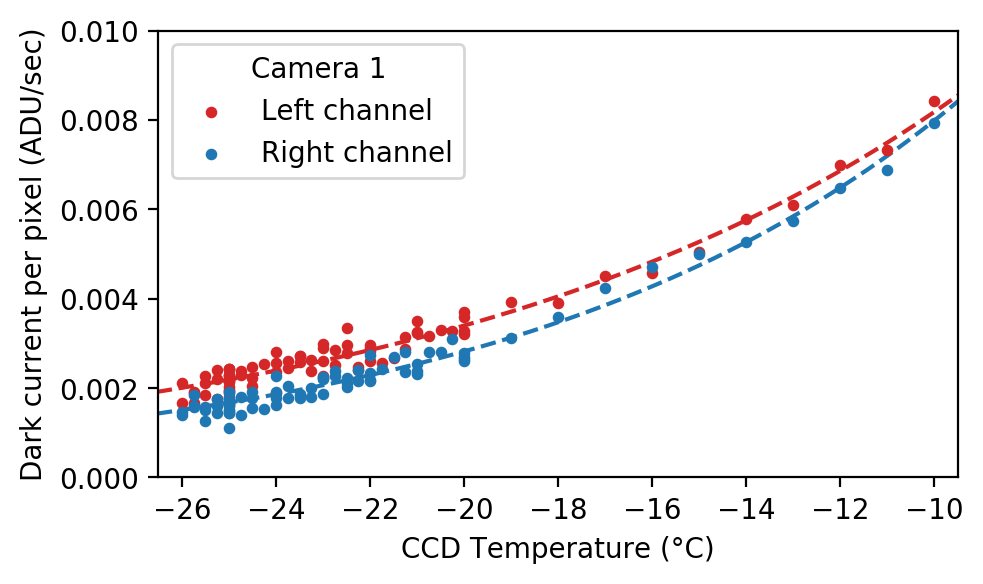
\includegraphics[width=\linewidth]{images/detectors/dc_1.png}
        \end{minipage}
        \begin{minipage}[t]{0.49\textwidth}\vspace{10pt}
            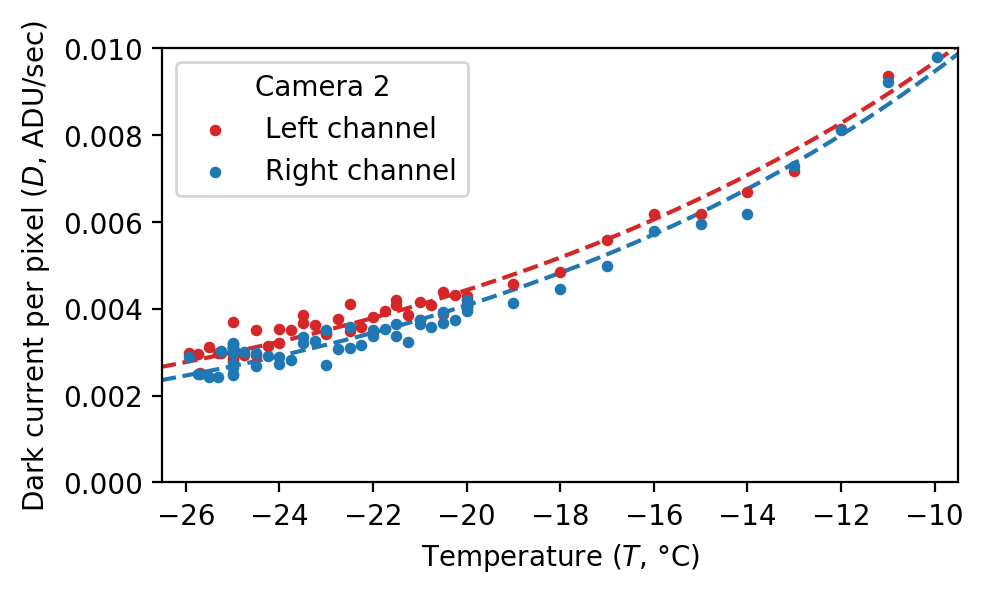
\includegraphics[width=\linewidth]{images/detectors/dc_2.png}
        \end{minipage}

        \begin{minipage}[t]{0.49\textwidth}\vspace{10pt}
            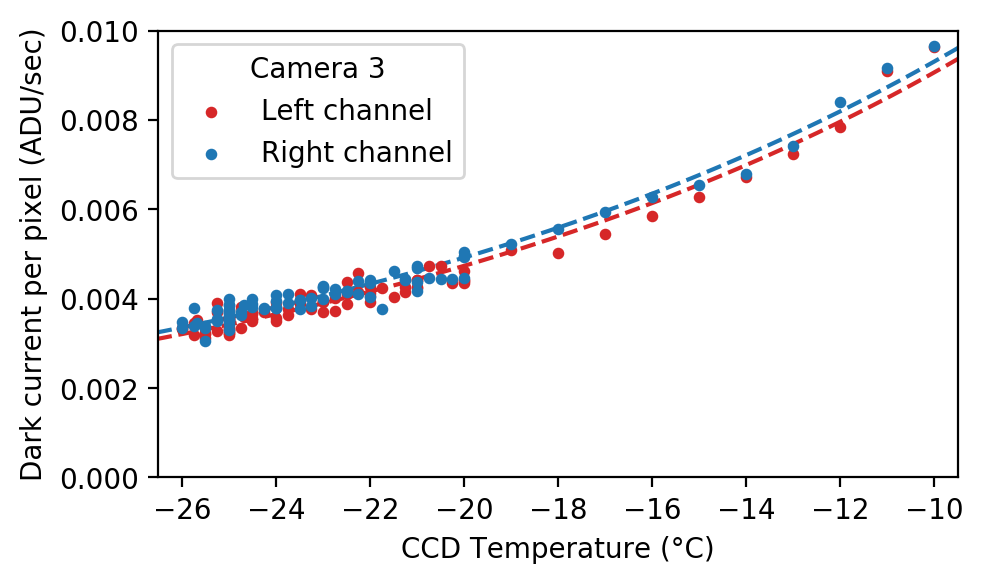
\includegraphics[width=\linewidth]{images/detectors/dc_3.png}
        \end{minipage}
        \begin{minipage}[t]{0.49\textwidth}\vspace{10pt}
            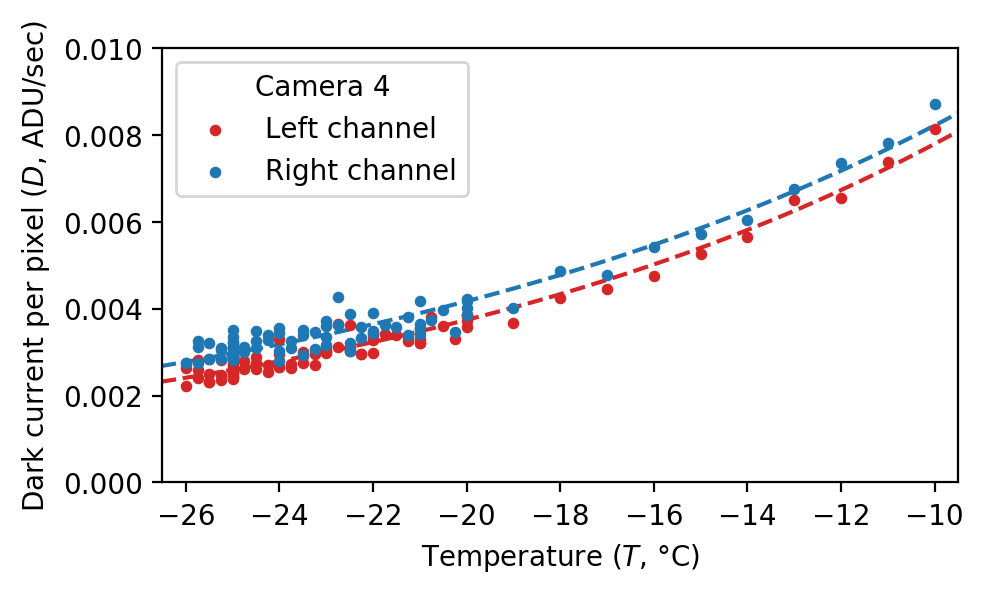
\includegraphics[width=\linewidth]{images/detectors/dc_4.png}
        \end{minipage}

        \begin{minipage}[t]{0.49\textwidth}\vspace{10pt}
            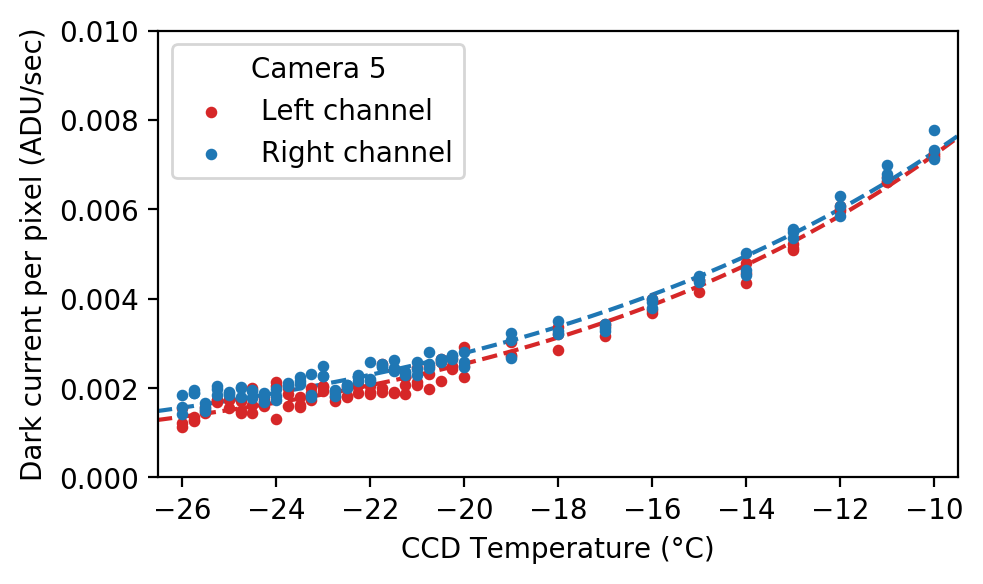
\includegraphics[width=\linewidth]{images/detectors/dc_5.png}
        \end{minipage}
        \begin{minipage}[t]{0.49\textwidth}\vspace{10pt}
            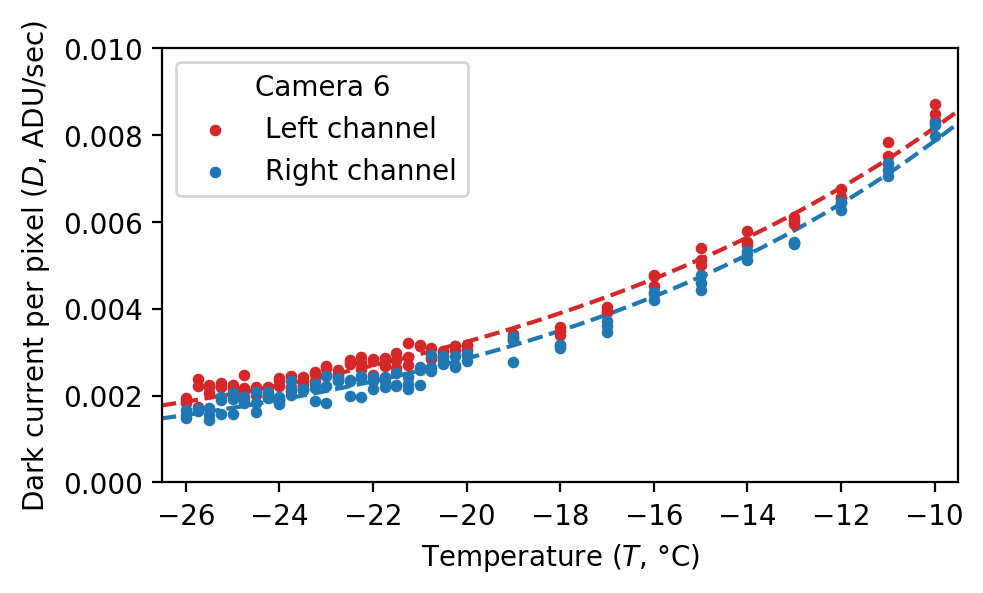
\includegraphics[width=\linewidth]{images/detectors/dc_6.png}
        \end{minipage}

        \begin{minipage}[t]{0.49\textwidth}\vspace{10pt}
            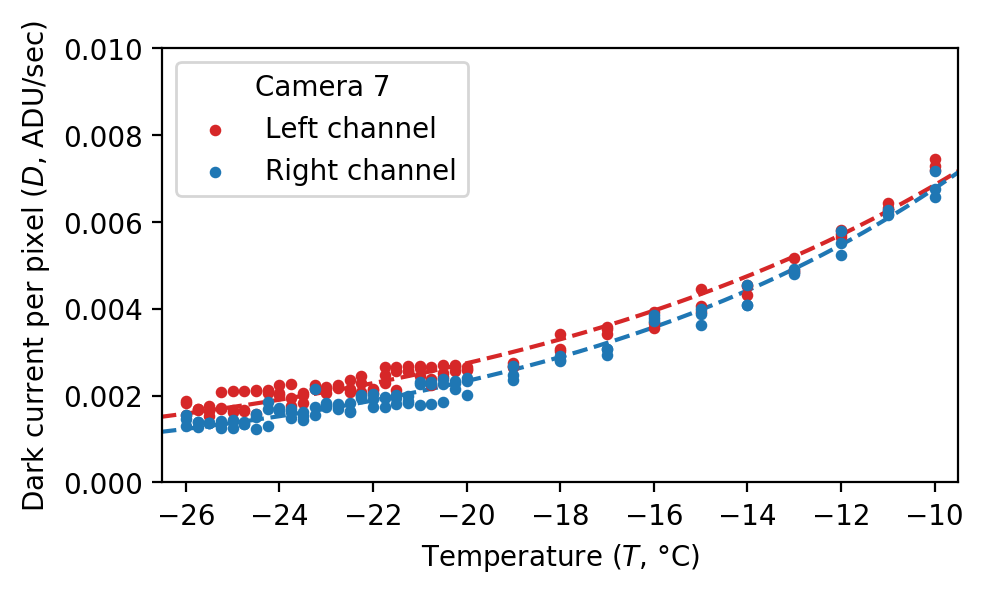
\includegraphics[width=\linewidth]{images/detectors/dc_7.png}
        \end{minipage}
        \begin{minipage}[t]{0.49\textwidth}\vspace{10pt}
            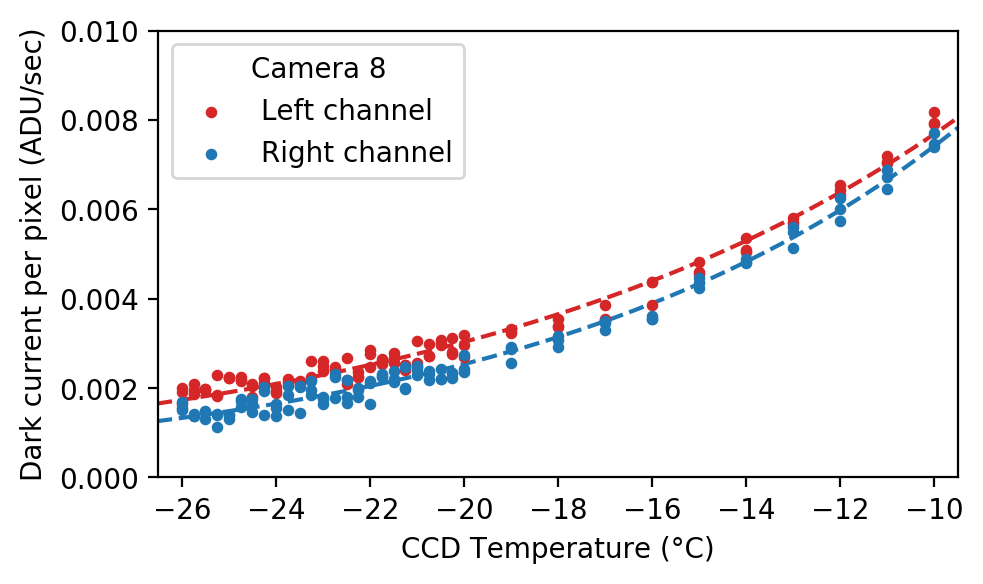
\includegraphics[width=\linewidth]{images/detectors/dc_8.png}
        \end{minipage}
    \end{center}
    \caption[Dark current plots]{
        Dark current plots for each camera.
    }\label{fig:dcs}
\end{figure}

\clearpage

\end{colsection}

% ~~~~~~~~~~~~~~~~~~~~
\newpage
\subsection{Linearity}
\label{sec:lin}
\begin{colsection}

Linearity is a measure of the response of the CCD over its dynamic range. It is particularly important for scientific imaging that the measured counts are directly proportional to the object signal.

The non-linearity of each camera was measured using the same images taken for the photon transfer curves in \aref{sec:ptc}, bright images of a flat source with increasing exposure times. The images were bias-subtracted, and the mean counts of a central 2000$\times$2000 pixel region in the centre of each channel was plotted against the exposure time, shown in \aref{fig:lin}. A linear relation was fitted to the central potion of the data, excluding the upper and lower 10\% of the dynamic range. Residuals from this fit as a percentage of the count are also plotted in \aref{fig:lin}, and the mean absolute deviation from the linear fit over the central region is given in \aref{tab:lin}.

The values for non-linearity measured vary greatly between each camera, and several are over 1\%. If these values were true this would be a major problem when making accurate photometric measurements. However, the FLI specification advertises a non-linearity of <1\%, and FLI's own tests of the cameras consistently report non-linearity of 0.2\% or less. Accurately measuring the response of a CCD requires a perfectly uniform light source and an integrating sphere, which FLI would have access to. I had to make do with a LCD screen when carrying out the tests in the lab, which is a poor substitute. Therefore the values in \aref{tab:lin} should not be considered reliable measurements.

\begin{table}[t]
    \begin{center}
        \begin{tabular}{c|cc} %chktex 44
             & \multicolumn{2}{c}{Non-linearity} \\
             & \multicolumn{2}{c}{(\%)} \\
             & \multicolumn{1}{c}{L} & \multicolumn{1}{c}{R} \\
            \midrule
            Camera 1 & 2.29 & 2.00 \\
            Camera 2 & 0.76 & 0.65 \\
            Camera 3 & 0.34 & 0.39 \\
            Camera 4 & 0.18 & 0.22 \\
        \end{tabular}
        \hspace{0.5cm}
        \begin{tabular}{c|cc} %chktex 44
             & \multicolumn{2}{c}{Non-linearity} \\
             & \multicolumn{2}{c}{(\%)} \\
             & \multicolumn{1}{c}{L} & \multicolumn{1}{c}{R} \\
            \midrule
            Camera 5 & 1.25 & 1.20 \\
            Camera 6 & 1.20 & 1.13 \\
            Camera 7 & 0.70 & 0.68 \\
            Camera 8 & 0.82 & 0.80 \\
        \end{tabular}
    \end{center}
    \caption[Non-linearity values]{
        Non-linearity values for each camera.
    }\label{tab:lin}
\end{table}

\begin{figure}[p]
    \begin{center}
        \begin{minipage}[t]{0.49\textwidth}\vspace{10pt}
            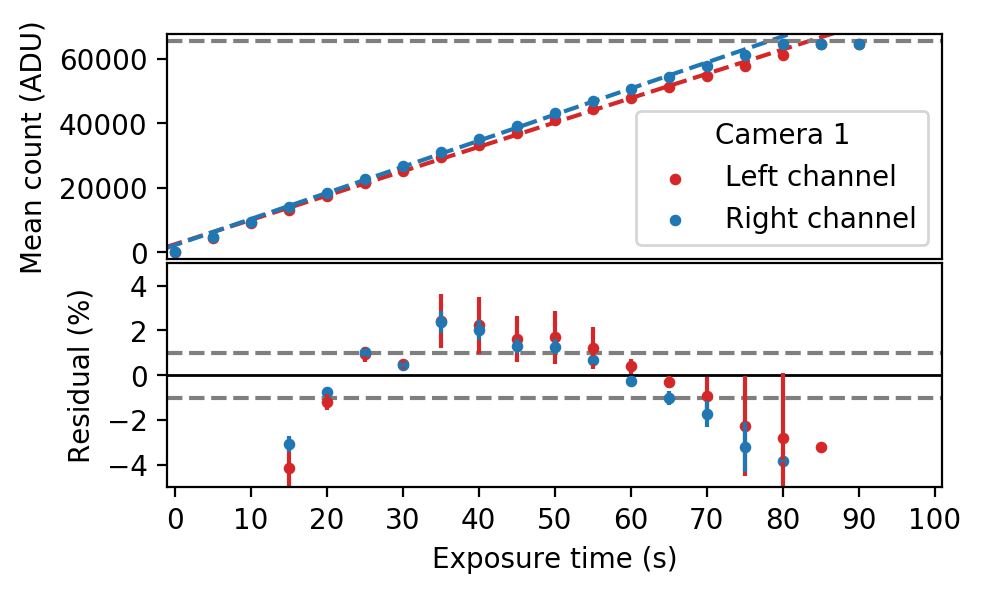
\includegraphics[width=\linewidth]{images/detectors/lin_1.png}
        \end{minipage}
        \begin{minipage}[t]{0.49\textwidth}\vspace{10pt}
            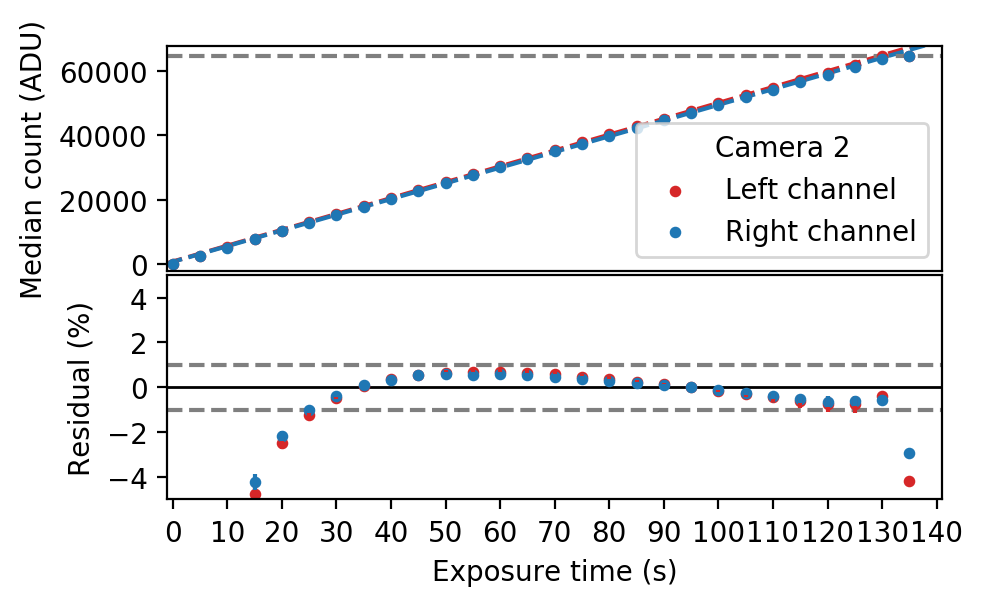
\includegraphics[width=\linewidth]{images/detectors/lin_2.png}
        \end{minipage}

        \begin{minipage}[t]{0.49\textwidth}\vspace{10pt}
            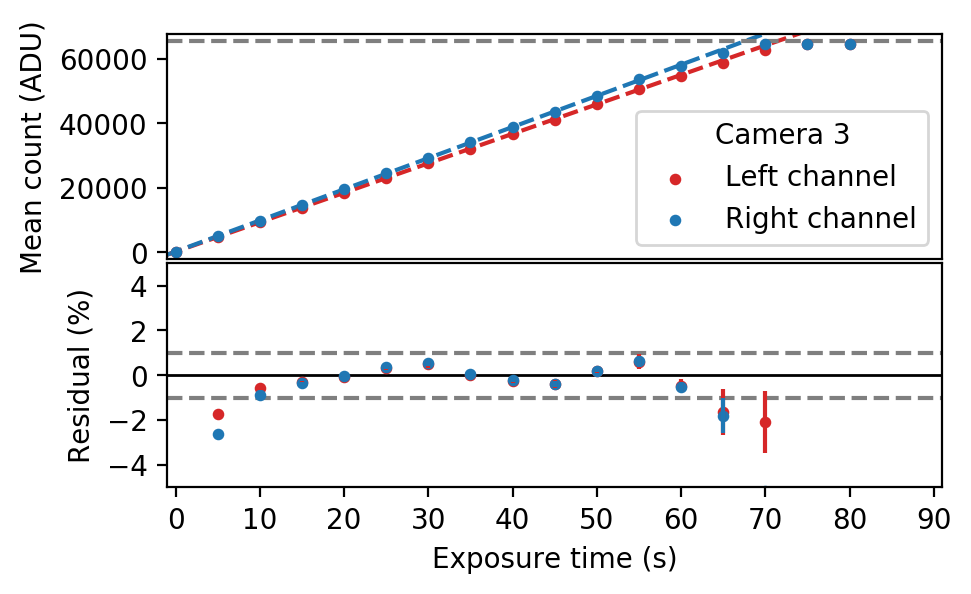
\includegraphics[width=\linewidth]{images/detectors/lin_3.png}
        \end{minipage}
        \begin{minipage}[t]{0.49\textwidth}\vspace{10pt}
            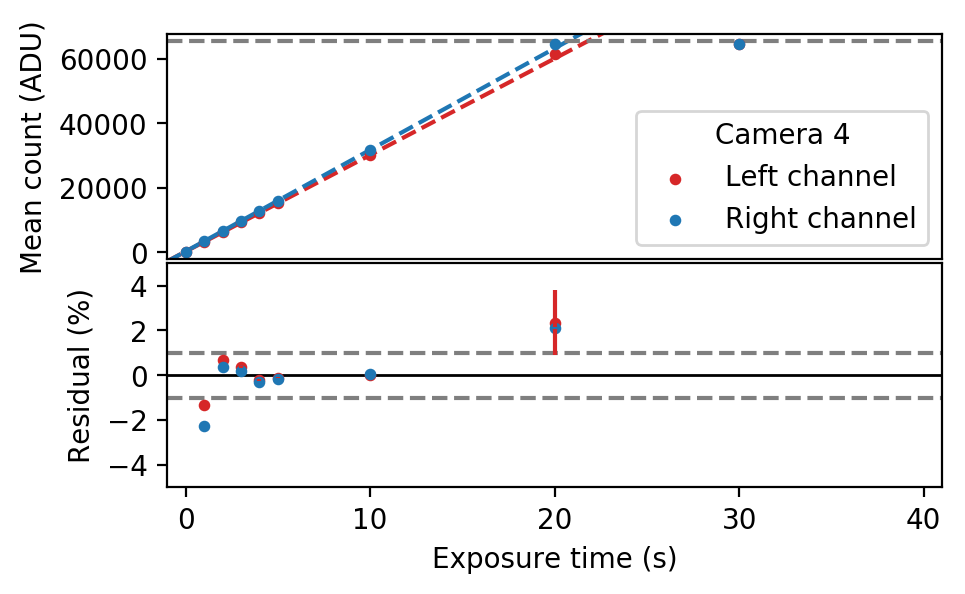
\includegraphics[width=\linewidth]{images/detectors/lin_4.png}
        \end{minipage}

        \begin{minipage}[t]{0.49\textwidth}\vspace{10pt}
            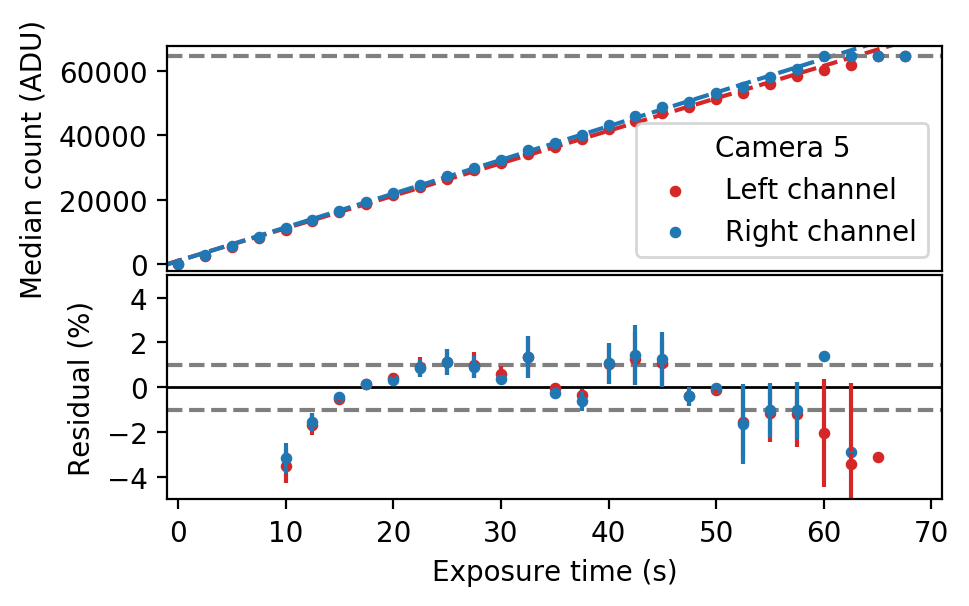
\includegraphics[width=\linewidth]{images/detectors/lin_5.png}
        \end{minipage}
        \begin{minipage}[t]{0.49\textwidth}\vspace{10pt}
            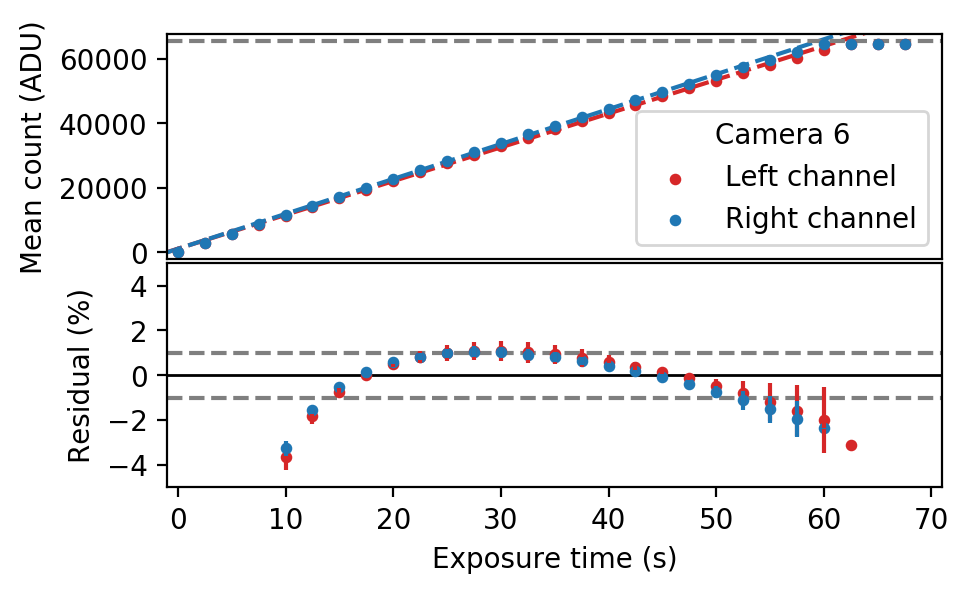
\includegraphics[width=\linewidth]{images/detectors/lin_6.png}
        \end{minipage}

        \begin{minipage}[t]{0.49\textwidth}\vspace{10pt}
            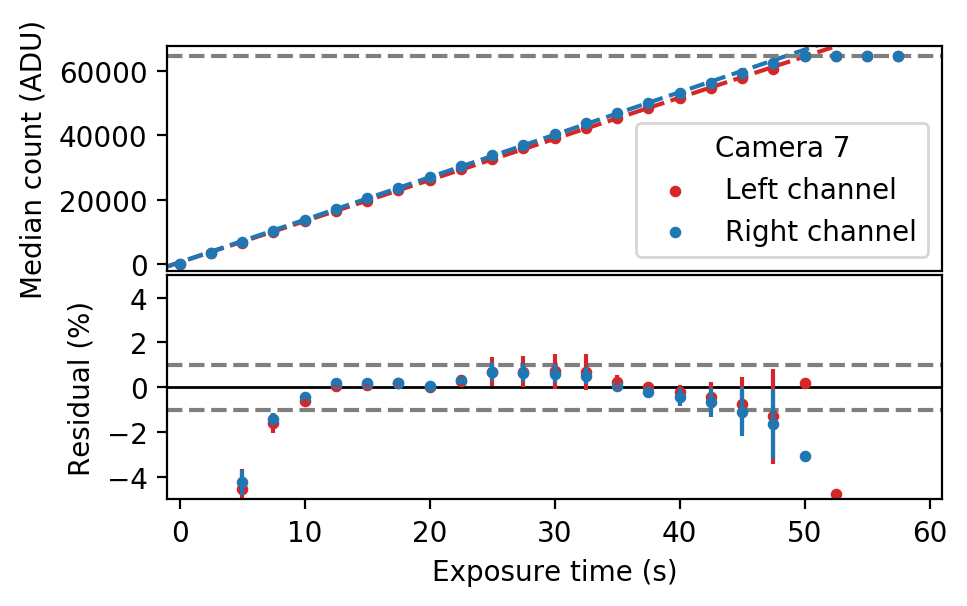
\includegraphics[width=\linewidth]{images/detectors/lin_7.png}
        \end{minipage}
        \begin{minipage}[t]{0.49\textwidth}\vspace{10pt}
            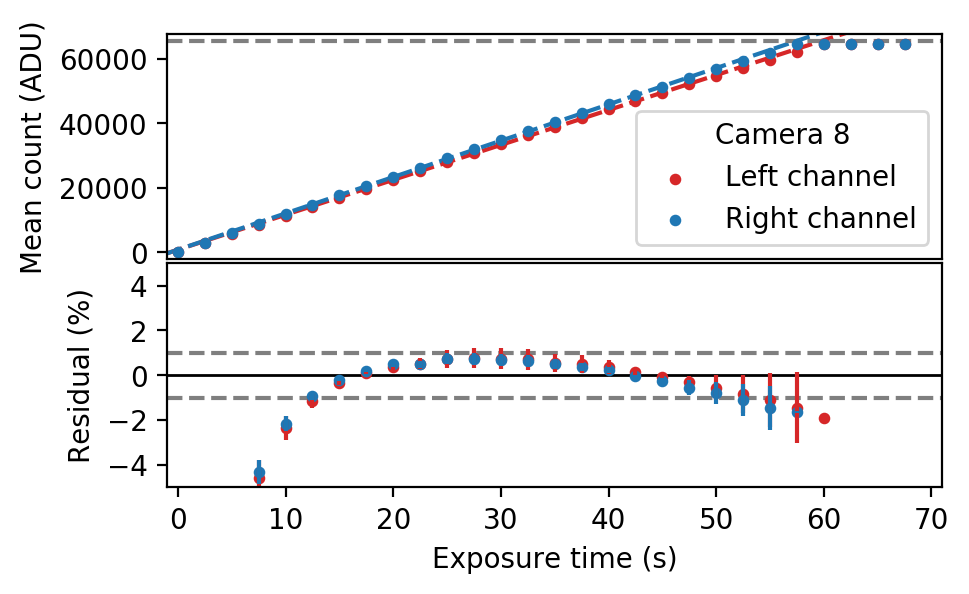
\includegraphics[width=\linewidth]{images/detectors/lin_8.png}
        \end{minipage}
    \end{center}
    \caption[Linearity plots]{
        Linearity plots for each camera.
    }\label{fig:lin}
\end{figure}

\clearpage

\end{colsection}

% ~~~~~~~~~~~~~~~~~~~~
\newpage
\subsection{Defects}
\label{sec:defects}
\begin{colsection}

There are several possible defects in CCD sensors \citep{CCDs}: hot pixels, which have atypically high dark currents, dead pixels, which produce zero counts, and trap pixels, which ``trap'' electrons and prevent read out from it and any pixels above it in the column. For targeted astronomical observations it is important to track any bad pixels, so whenever possible photons from the target object does not fall on any of them. GOTO's wide-field survey observations make this less of an issue, but the pipeline will track bad pixels and columns when calibrating images from each camera.

Single hot or dead pixels are not a major problem, as they can be removed by subtracting bias frames and flat fielding. If necessary the value of the bad pixel can be interpolated from the surrounding pixels. Trap pixels are more of an issue, as they take out the entire column behind them. For each camera a defect mask was made by taking the ratio of two flat images with different exposure times, making any bad pixels or columns easy to pick out by comparing to the surrounding pixels. And example of a trap pixel is shown in \aref{fig:itsatrap}. The positions of trap pixels for each camera are given in \aref{tab:traps}. The KAF-50100 chip specification gives an allowed limit of less than 20 column defects per device, which the GOTO cameras are well within.

\begin{table}[t]
    \begin{center}
        \begin{tabular}{c|ccc} %chktex 44
             & \multicolumn{2}{c}{Trap location} & Lost \\
             & x & y & \% \\
            \midrule
            Camera 1 & 7751 & 4361 & 30 \\
            Camera 2 & 1658 & ~172 & 97 \\ %chktex 39
            Camera 3 & 1224 & 1844 & 70 \\
                     & 5058 & 5185 & 17 \\
            Camera 4 & 5406 & 2607 & 58 \\
            Camera 5 & 6293 & 1416 & 77 \\
            Camera 6 & 5455 & 5036 & 19 \\
        \end{tabular}
        \hspace{0.5cm}
        \begin{tabular}{c|ccc} %chktex 44
            & \multicolumn{2}{c}{Trap location} & Lost \\
            & x & y & \% \\
            \midrule
            Camera 7 & 1344 & 3037 & 51 \\
                     & 2326 & 2495 & 60 \\
                     & 2610 & 5688 & ~9 \\ %chktex 39
                     & 7491 & 5120 & 18 \\
            Camera 8 & 1184 & 3043 & 51 \\
                     & 5659 & 2778 & 55 \\
            \multicolumn{4}{c}{} \\
        \end{tabular}
    \end{center}
    \caption[Locations of trap pixels]{
        Locations of trap pixels and fraction of the column lost for each camera.
    }\label{tab:traps}
\end{table}

\begin{figure}[p]
    \begin{center}
        \includegraphics[width=\textwidth]{images/detectors/defect_plot.pdf}
    \end{center}
    \caption[An example of a trap pixel]{
        A flat frame for Camera 1 showing an example of a trap pixel. The plot below of counts averaged in the y axis clearly shows the bad column, and the depth of the well beneath the field level is proportional to the height of the trap pixel in the column.
    }\label{fig:itsatrap}
\end{figure}

\clearpage

\end{colsection}

% ~~~~~~~~~~~~~~~~~~~~

\end{colsection}

% ########################################

\newpage
\section{System throughput}
\label{sec:throughput}
\begin{colsection}

% ~~~~~~~~~~~~~~~~~~~~

\begin{colsection}

Unfortunately, not every photon emitted by a target object will reach our cameras. Photons will be lost due to the finite transmittance of the telescope optics, and before that a certain fraction of light will be lost due to extension in the atmosphere. Understanding each element is required in order to produce a complete throughput model.

\end{colsection}

% ~~~~~~~~~~~~~~~~~~~~
\subsection{Optical elements}
\label{sec:optics}
\begin{colsection}

The GOTO unit telescopes are Wynne-Newtonian astrographs: fast (f/2.5) Newtonian telescopes with a \SI{40}{\centi\meter} primary mirror, a flat elliptical secondary (\SI{19}{\centi\metre} short axis) and a three-lens Wynne corrector between the secondary mirror and camera to focus light back onto the CCD detector. The full \gls{ota} design is shown in \aref{fig:ota}, and the five elements the light must pass through (the three corrector lenses, the filter in the filter wheel and the window in front of the detector) are shown in \aref{fig:wynne}. In order to correctly model the throughput each element needed to be considered in turn.

% ---------
\subsubsection{Mirrors}

The GOTO mirrors are made of coated aluminium, and were manufactured by Orion Optics\footnote{\url{https://www.orionoptics.co.uk/}}. Orion uses their own ``HiLux'' high reflectivity coating, and while individual reflectance curves were not available for the GOTO mirrors at the time this work was carried out Orion does provide a representative reflectance curve on their website (shown in \aref{fig:trans_ota}). As there are two mirrors this curve will be included twice in the final throughput model. Orion's website states that the difference in angle of incidence of the two mirrors is accounted for in the thickness of the coating applied, so otherwise the two mirrors can be treated as identical.

\newpage

\begin{figure}[p]
    \begin{center}
        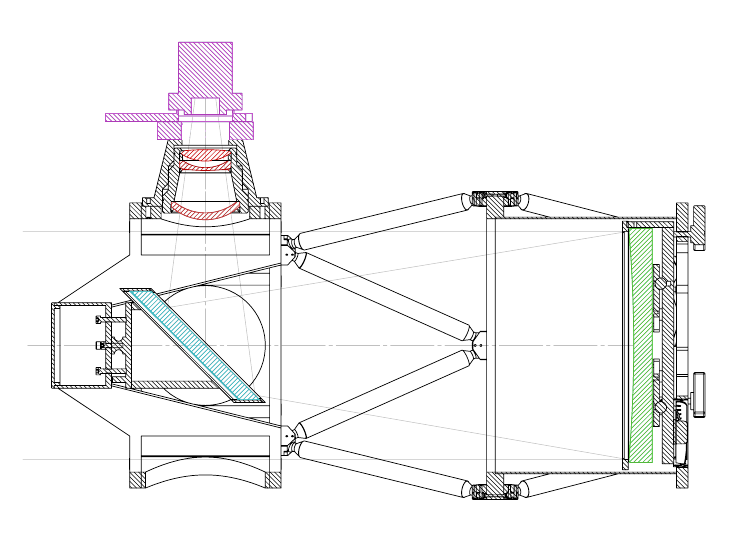
\includegraphics[width=0.7\textwidth]{images/throughput/OTA_optics.png}
    \end{center}
    \caption[GOTO optical telescope assembly]{
        The \gls{ota} design for one of the GOTO prototype unit telescopes. Light enters from the left, and the optical elements have been highlighted: the primary mirror in \textcolorbf{Green}{green}, the secondary mirror in \textcolorbf{BlueGreen}{blue}, the Wynne corrector lenses in \textcolorbf{Red}{red} and the FLI camera hardware (focuser, filter wheel and camera) in \textcolorbf{Purple}{purple}.
    }\label{fig:ota}
\end{figure}

\begin{figure}[p]
    \begin{center}
        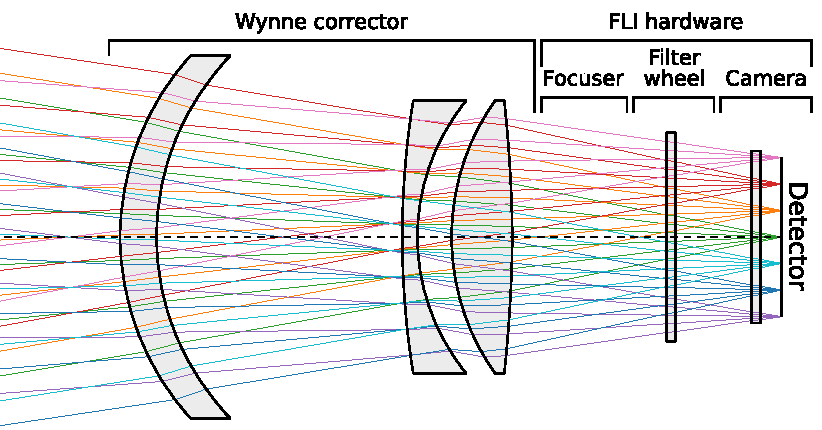
\includegraphics[width=0.7\textwidth]{images/throughput/wynne.pdf}
    \end{center}
    \caption[Ray tracing the corrector elements]{
        A ray trace showing the optical elements after the secondary mirror. From left-to-right light passes through the three Wynne corrector lenses, the focuser (which contains no optical elements), the filter in the filter wheel and the camera window before reaching the detector located in the focal plane.
    }\label{fig:wynne}
\end{figure}

\clearpage

% ---------
\subsubsection{Lenses}

\begin{table}[t]
    \begin{center}
        \begin{tabular}{c|cccc} %chktex 44
            Lens & Type     & Glass (manufacturer) & Diameter               & On-axis thickness \\
            \midrule
               1 & Crescent &    H-K9L (Schott)    & \SI{120}{\milli\meter} & \SI{12}{\milli\meter} \\
               2 & Crescent &    H-K9L (Schott)    & \SI{90}{\milli\meter}  & \SI{5}{\milli\meter} \\
               3 & Biconvex &  S-FPL53 (Ohara)     & \SI{90}{\milli\meter}  & \SI{20}{\milli\meter} \\
        \end{tabular}
    \end{center}
    \caption[Wynne corrector lens properties]{
        Properties of the three Wynne corrector lenses.
    }\label{tab:lenses}
\end{table}

Each Wynne corrector contains three lenses, as shown in \aref{fig:wynne}, and the physical details of each lens are given in \aref{tab:lenses}. No complete transmission data was available, so a model throughput curve was created.

Both the reflectivity of the front surface and the internal transmittance of the lens glass needs to be considered. Each lens was coated with an anti-reflection coating, the profile of which was included in the GOTO optical report. Transmittance curves for each lens were not available, however the glass types were included in the report and are given in \aref{tab:lenses}. Transmittance data provided by the manufacturers was retrieved from the online Refractive Index Database\footnote{\url{https://refractiveindex.info/}}. For simplicity each lens was modelled as having a constant thickness, using their on-axis thickness. As shown in \aref{fig:wynne} this is true for lens 1 but will typically underestimate the thickness of lens 2 and overestimate the thickness of lens 3. However the thickness of glass each light path travels through should be the same, and as there is very little difference between the two types of glass the overall throughput will be approximately the same.

Throughput curves for the anti-reflection coating and the three lenses are shown in \aref{fig:trans_lenses}, along with the total throughput found by multiplying the contribution from the glass and coating for each lens.

\newpage

\begin{figure}[t]
    \begin{center}
        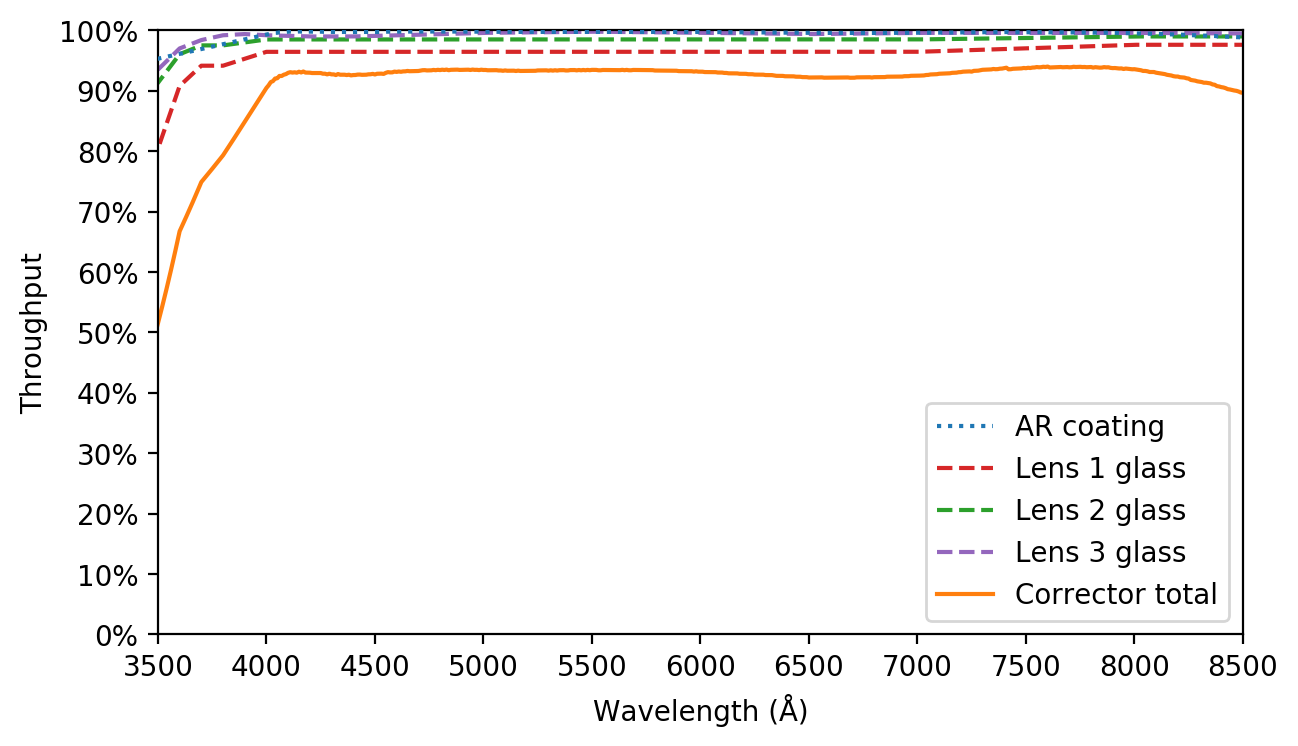
\includegraphics[width=\textwidth]{images/throughput/trans_lenses.png}
    \end{center}
    \caption[Wynne corrector transmission curve]{
        Transmission curve for the Wynne corrector, comprised of the three lenses each with an anti-reflection (AR) coating.
    }\label{fig:trans_lenses}
\end{figure}

% ---------
\subsubsection{Filters}

The filter transmittance is included in their bandpass profiles, described below in \aref{sec:filters}. At this stage we will consider the \gls{ota} with no filter in place.

% ---------
\subsubsection{Camera window}

Finally, before reaching the detector light must pass through a glass window in the camera which protects the CCD sensor. The window is made of F116 glass, and a transmission profile was provided by FLI.\@ This is shown in \aref{fig:trans_ota}.

\newpage

% ---------
\subsubsection{Combined OTA throughput}

The combined throughput for the whole unfiltered OTA is shown in \aref{fig:trans_ota}. This was constructed by multiplying through the transmission curves for the two mirrors, the corrector and the camera window. In the 4000--\SI{7000}{\angstrom} visible region used by GOTO the throughput is typically 60\% or above, although all the elements have a sharp cut-off towards the UV at low wavelengths.

\begin{figure}[t]
    \begin{center}
        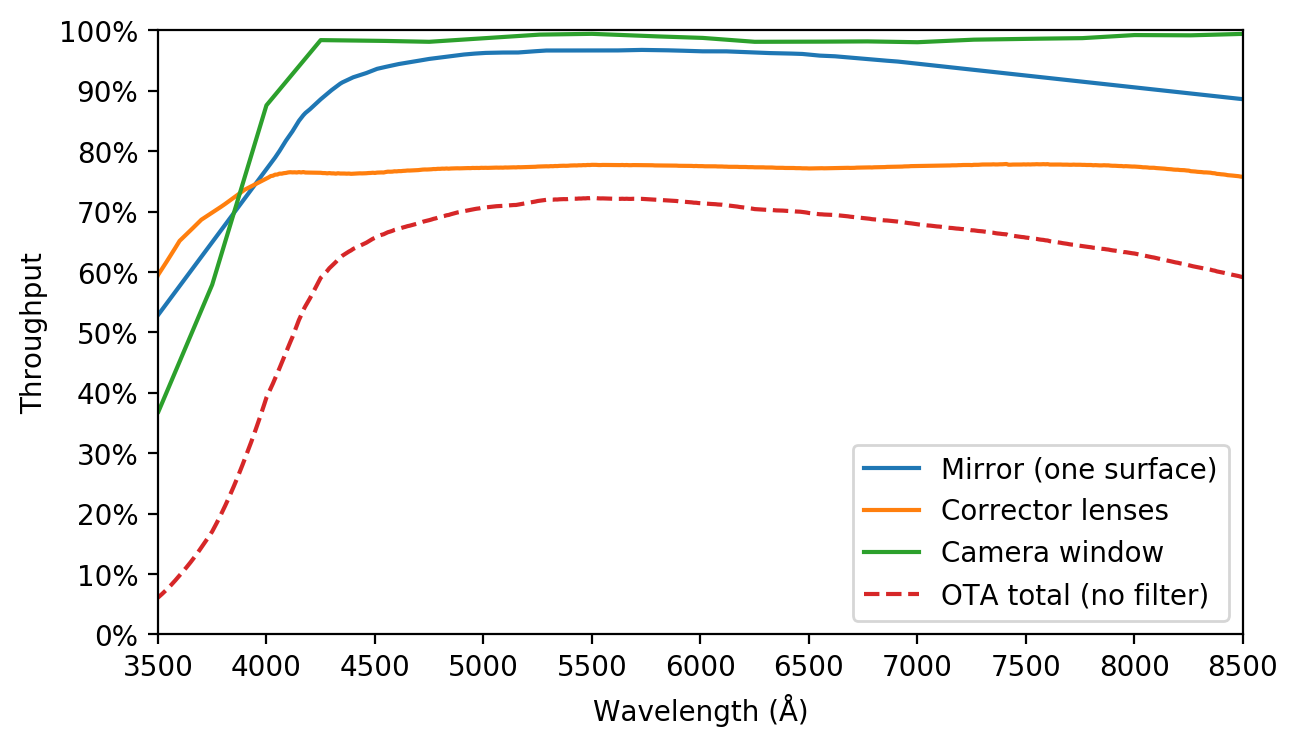
\includegraphics[width=\textwidth]{images/throughput/trans_ota.png}
    \end{center}
    \caption[Combined OTA transmission curve]{
        Transmission curve for the unfiltered OTA, including two mirrors, the corrector lenses and the camera window.
    }\label{fig:trans_ota}
\end{figure}

\end{colsection}

% ~~~~~~~~~~~~~~~~~~~~
\newpage
\subsection{Filters}
\label{sec:filters}
\begin{colsection}

\begin{figure}[t]
    \begin{center}
        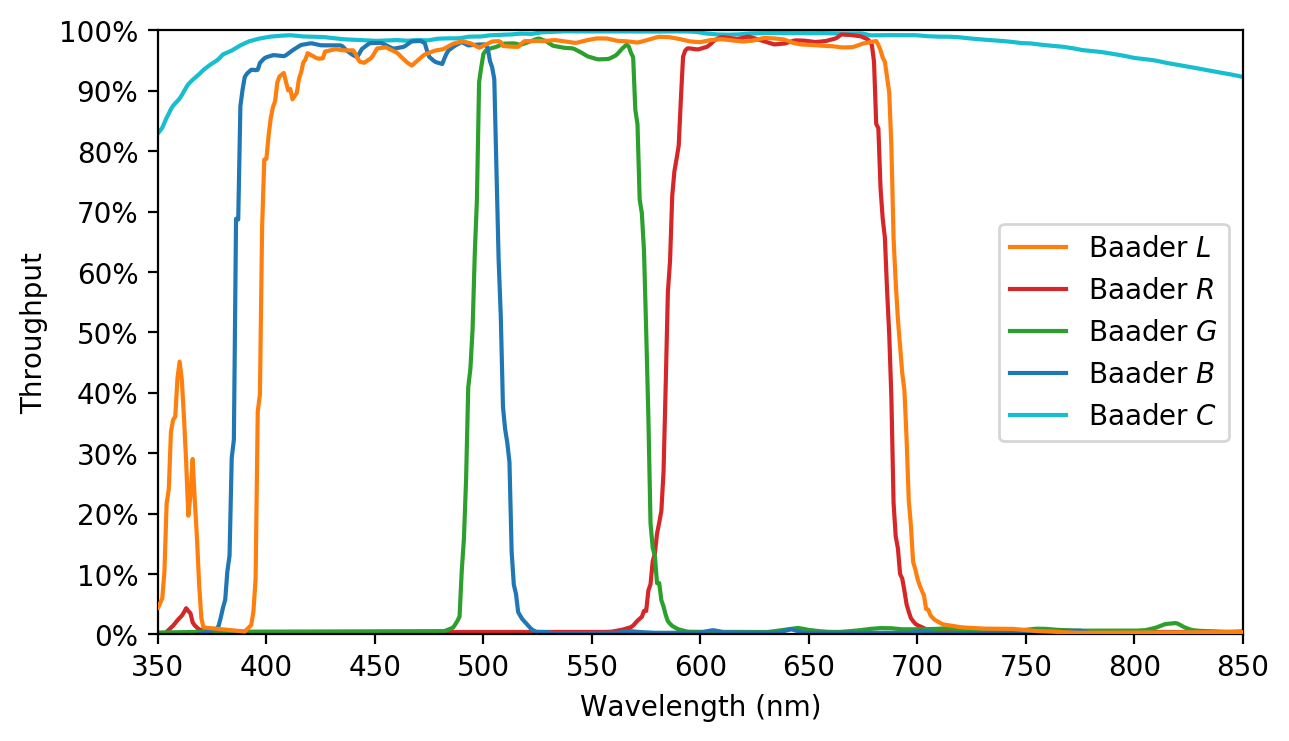
\includegraphics[width=\textwidth]{images/throughput/trans_filters.png}
    \end{center}
    \caption[Baader filter transmission curves]{
        Transmission curves for the Baader \textit{LRGBC} filter set used by GOTO.\
    }\label{fig:filters}
\end{figure}

Each GOTO unit telescope has a five-slot CFW9--5 filter wheel from FLI.\@ Each contains a set of \SI{65}{\milli\metre} square filters from Baader Planetarium\footnote{\url{https://www.baader-planetarium.com/}}: three coloured filters (\textit{R}, \textit{G}, \textit{B}), one wide ``luminance'' filter (\textit{L}) covering the whole visible range, and a clear glass filter ({\textit{C}}). Transmission curves for each filter are shown in \aref{fig:filters}. Each filter has a high throughput and steep cut-offs outside of the desired bandpasses. For the coloured filters the cut-offs were chosen so the [O\textsc{iii}] $\lambda 5007$ emission line falls within the overlap of the \textit{B} and \textit{G} filters and the region around \SI{5800}{\angstrom}, which contains emission lines from Mercury and Sodium vapour lamps, is excluded by the gap between the \textit{G} and \textit{R} filters.

The clear filter is never used for scientific observations, so from now on only the \textit{LRGB} filters are considered. Most of GOTO observations are taken using the \textit{L} filter, because it would currently take too long to survey in multiple colours. However the \textit{RBG} filters have been used for targeted observations and manual follow-up images.

\begin{table}[t]
    \begin{center}
        \begin{tabular}{c|cccc} %chktex 44
            Filter            & Central wavelength                          & Bandwidth            \\
             & ($\lambda_\text{eff}$, \SI{}{\angstrom}) & ($\Delta\lambda$, \SI{}{\angstrom}) \\
            \midrule
            Baader \textit{L} & 5355 & 2942 \\
            Baader \textit{R} & 6573 &  979 \\
            Baader \textit{G} & 5373 &  813 \\
            Baader \textit{B} & 4509 & 1188 \\
        \end{tabular}
    \end{center}
    \caption[Baader filter properties]{
        Properties of the Baader \textit{LRGB} filters.
    }\label{tab:filters}
\end{table}

Properties of the four \textit{LRGB} filters are given in \aref{tab:filters}. The effective wavelength $\lambda_\text{eff}$ given is the pivot wavelength as defined in \citet{HST_calibration} for HST filters

\begin{equation}
    \lambda_\text{eff}^2 = \frac{\int T\lambda \, d\lambda}{\int T/\lambda \, d\lambda},
    \label{eq:pivot_wavelength}
\end{equation}

where $T$ is the transmission integrated over all wavelengths $\lambda$. The effective bandwidth $\Delta\lambda$ is defined as the width of a rectangle that has a height of the maximum transmission (1) and the same area as the area under the filter transmission curve, i.e.

\begin{equation}
    \Delta\lambda = \int T d\lambda.
    \label{eq:bandwidth}
\end{equation}

GOTO uses the Baader filters primarily based on cost, as each complete mount would require 8 filter sets. The Baader filters were designed for amateur astronomers and astro-photographers and are less common for scientific instruments than other sets; such as the \textit{u'g'r'i'z'} set used by the Sloan Digital Sky Survey \citep{Sloan_filters}, or the traditional Johnson-Cousins \textit{UBVRI} set redefined in \citet{Bessell_filters}. A comparison of the transmission curves are shown in \aref{fig:filter_comparison1} for Sloan and \aref{fig:filter_comparison2} for Bessell. As can be seen the Baader \textit{L} filter approximately covers the extent of the Sloan \textit{g'} and \textit{r'}, with the \textit{B} and \textit{G} filters covering \textit{g'} and \textit{R} roughly matching \textit{r'}. Colour terms to compare GOTO \textit{RBG} observations with others using the Sloan \textit{g'} and \textit{r'} filters were calculated in \citet{Phaethon}.

\newpage

\begin{figure}[t]
    \begin{center}
        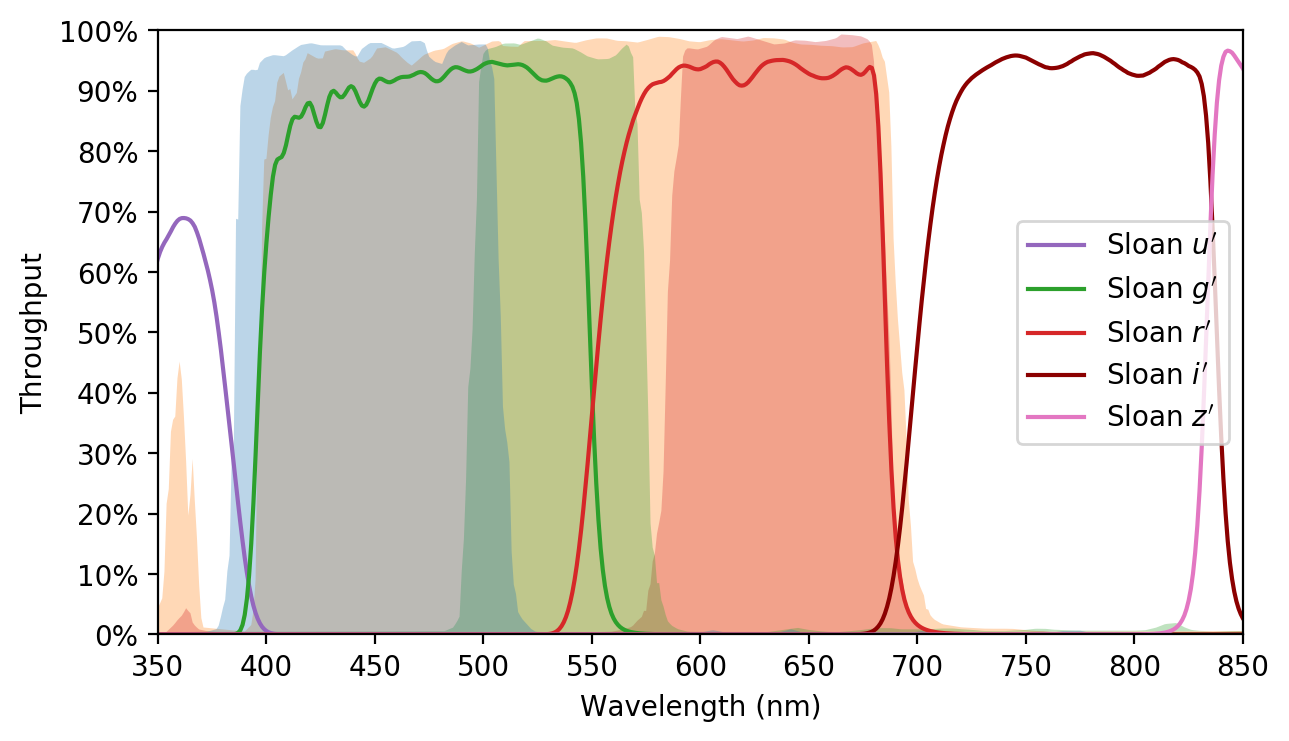
\includegraphics[width=\textwidth]{images/throughput/filt_comp1.png}
    \end{center}
    \caption[Comparison of Baader and Sloan filters]{
        A comparison of the Baader \textit{LRGB} filters to the Sloan \textit{u'g'r'i'z'} set.
    }\label{fig:filter_comparison1}
\end{figure}

\begin{figure}[t]
    \begin{center}
        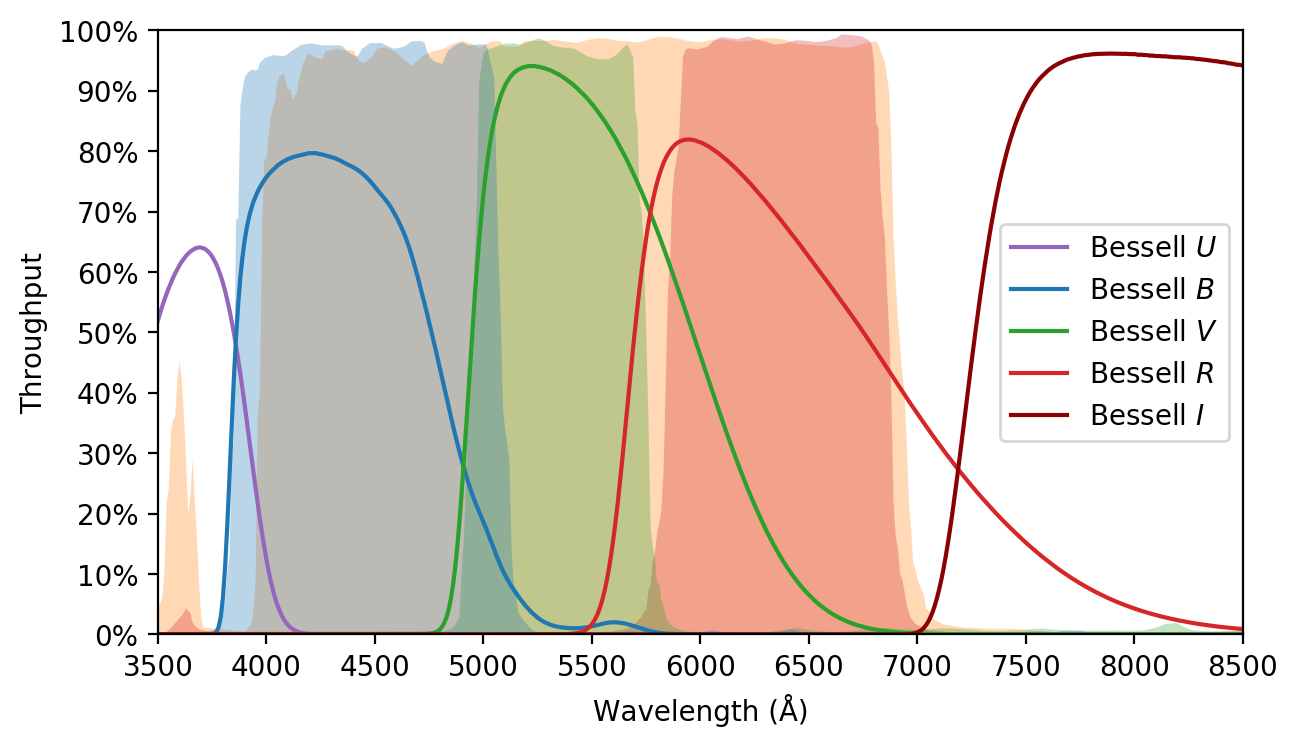
\includegraphics[width=\textwidth]{images/throughput/filt_comp2.png}
    \end{center}
    \caption[Comparison of Baader and Bessell filters]{
        A comparison of the Baader \textit{LRGB} filters to the Bessell \textit{UBVRI} set.
    }\label{fig:filter_comparison2}
\end{figure}

\clearpage

\end{colsection}

% ~~~~~~~~~~~~~~~~~~~~
\newpage
\subsection{Atmospheric extinction}
\label{sec:atmosphere}
\begin{colsection}

In order to fully model light from an astronomical source through to the CCD detector the absorption of light by the Earth's atmosphere must also be considered. The atmosphere is close to transparent over most of the visible region, however losses due to Rayleigh scattering begin to dominate closer to the UV \citep{atmosphere}.

The amount of light lost due to absorption and scattering in the atmosphere will depend on the altitude of the source, as light from sources closer to the horizon will pass through more atmosphere. The transmission of the atmosphere above La Palma has been measured as a function of airmass in \citet{tn31}, and is shown in \aref{fig:trans_atm}.

\begin{figure}[t]
    \begin{center}
        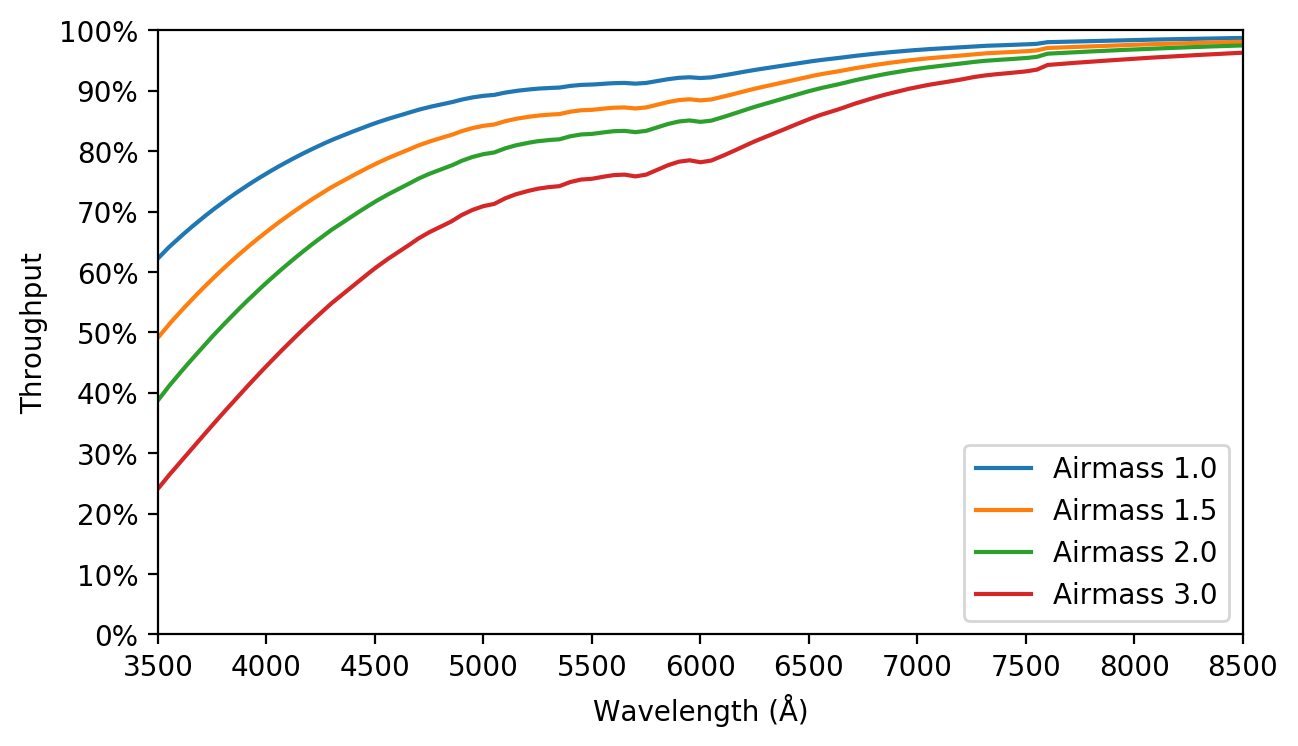
\includegraphics[width=\textwidth]{images/throughput/trans_atm.png}
    \end{center}
    \caption[Atmospheric transmission curve]{
        Transmission curve for the atmosphere at several airmasses.
    }\label{fig:trans_atm}
\end{figure}

\end{colsection}

% ~~~~~~~~~~~~~~~~~~~~
\newpage
\subsection{Quantum efficiency}
\label{sec:qe}
\begin{colsection}

\begin{figure}[t]
    \begin{center}
        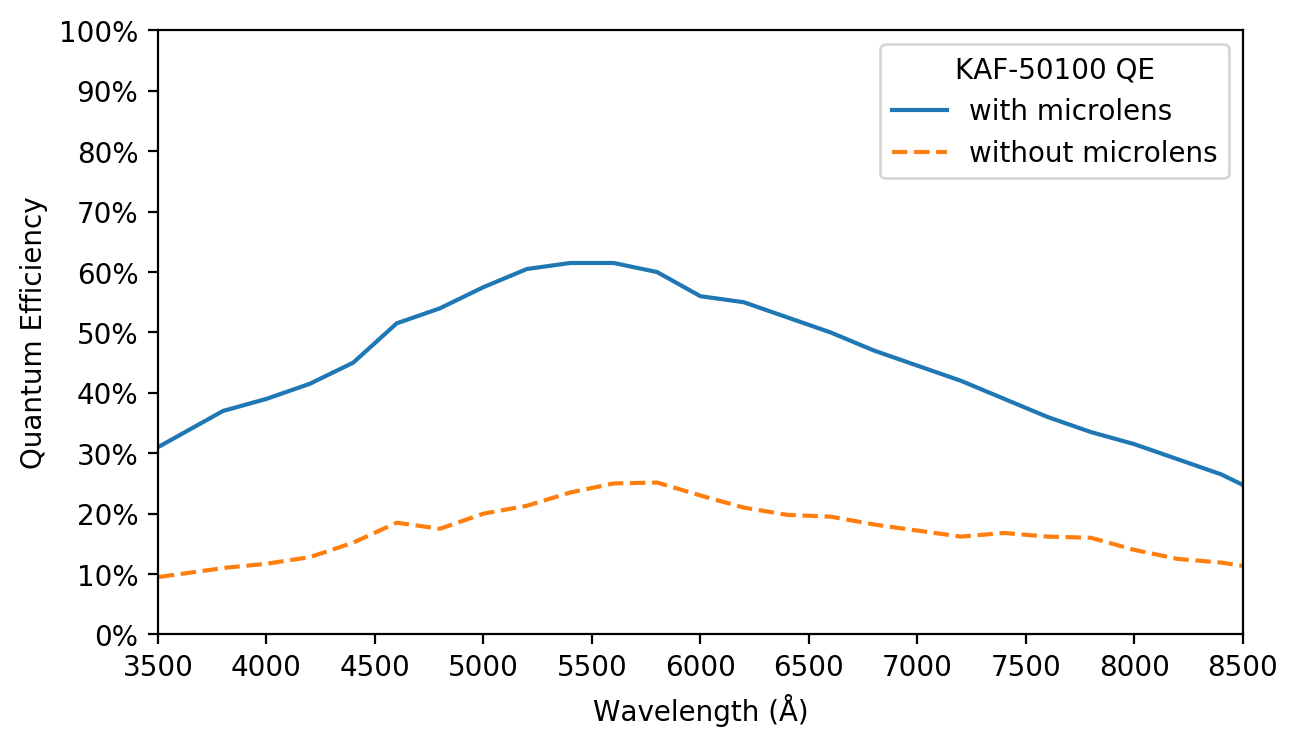
\includegraphics[width=\textwidth]{images/throughput/qe.png}
    \end{center}
    \caption[MicroLine quantum efficiency curve]{
        Quantum efficiency curve for the GOTO MicroLine cameras.
    }\label{fig:qe}
\end{figure}

Once photons pass through the atmosphere and the telescope they are focused onto the CCD, where they interact with the photosensitive layer and produce electric charge carriers which are recorded by the detector \citep{CCDs}. The conversion from photons to electrons is measured by the \gls{qe} of the CCD and is dependent on wavelength: short-wavelength photons will be absorbed before reaching the photosensitive layer, while long wavelength photons will not have enough energy to create free electrons from the silicon. The QE curve for the front-illuminated KAF-50100 CCDs within the GOTO MicroLine cameras was provided by FLI, and is shown in \aref{fig:qe}. CCDs that are back-side illuminated have improved QE as each photon passes through fewer layers and therefore has less chance of being absorbed, however these are more complicated and expensive to build. The quantum efficiency of a CCD can also change as a function of temperature, but this is negligible in the visible portion of the spectrum. % The QE peaks at 60\% at \SI{5500}{\angstrom} and falls below 30\% outside of the visible region.

\end{colsection}

% ~~~~~~~~~~~~~~~~~~~~
\newpage
\subsection{Total throughput}
\label{sec:total_throughput}
\begin{colsection}

The complete GOTO throughput is a combination of all of the above elements. Each source profile was linearly extrapolated to fit the same wavelength range (3500--\SI{8500}{\angstrom}) and multiplied together to produce the complete throughput model, shown in \aref{fig:throughput}. As the quantum efficiency is included the throughput describes the conversion between photons entering the atmosphere to electrons detected in the CCD, and using with the gain values given in \aref{tab:ptc} the full conversion between source photons and output counts can be made. The mean throughput in each filter can be found by dividing the filled areas in \aref{fig:throughput} by the area of the filter bandpass, these are given in electrons per photon in \aref{tab:throughput_zeropoint} in the next section.

\begin{figure}[t]
    \begin{center}
        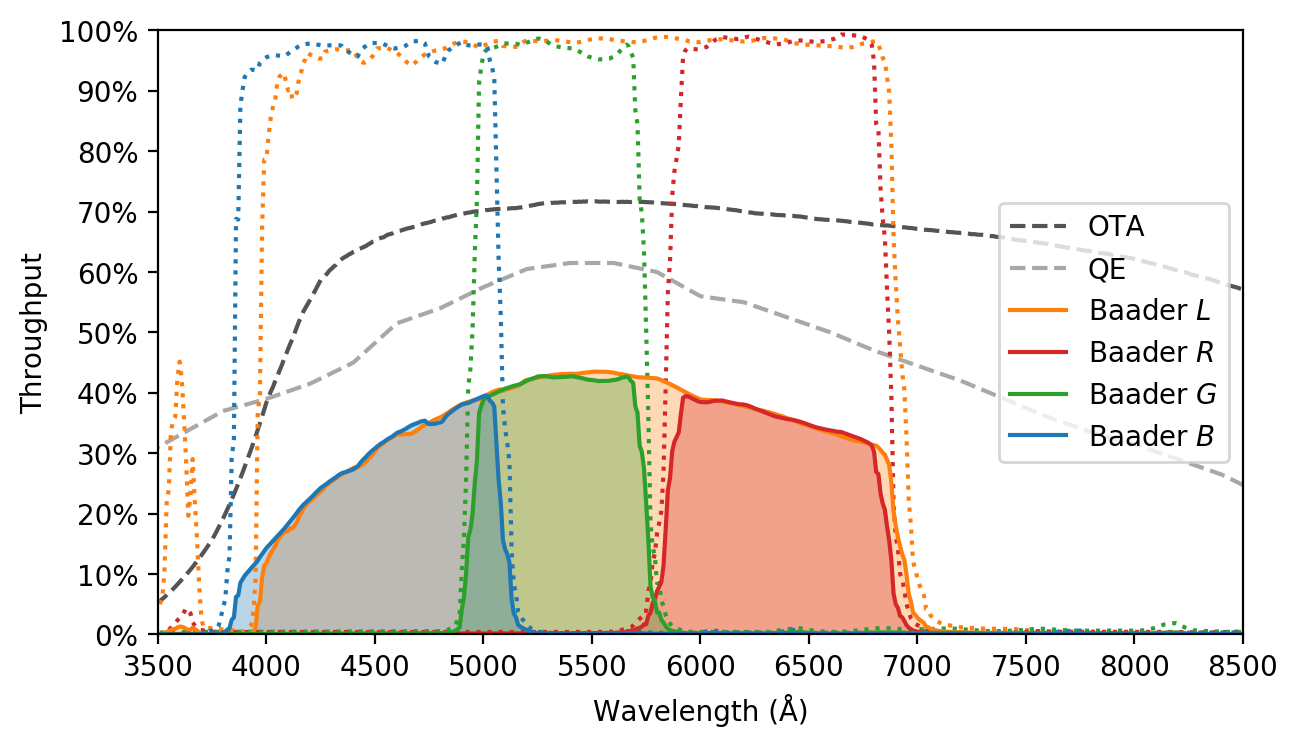
\includegraphics[width=\textwidth]{images/throughput/throughput.png}
    \end{center}
    \caption[Complete throughput model for the GOTO filters]{
        The complete GOTO throughput model for the Baader \textit{LRGB} filters (bandpasses from \aref{fig:filters}). Other contributions are from atmospheric extinction (from \aref{fig:trans_atm}, here assuming a source at zenith), throughput of the OTA elements (from \aref{fig:trans_ota}) and the quantum efficiency of the cameras (from \aref{fig:qe}).
    }\label{fig:throughput}
\end{figure}

\end{colsection}

% ~~~~~~~~~~~~~~~~~~~~

\end{colsection}

% ########################################

\newpage
\section{Photometric modelling}
\label{sec:photometry}
\begin{colsection}

% ~~~~~~~~~~~~~~~~~~~~

\begin{colsection}

Using the throughput model created in the previous section it is possible to simulate photometric observations with GOTO before the telescope was even commissioned. This section applies the theoretical model to two important photometric properties: the magnitude zeropoint, the correction required to convert between instrumental and ``real'' magnitude values, and the limiting magnitude, the brightest magnitude a source can bbe to still produce a noticeable signal above a given noise threshold. These theoretical values are then compared to values calculated from real GOTO observations in order to test the validity of the model and check that the hardware is performing to specification.

\end{colsection}

% ~~~~~~~~~~~~~~~~~~~~
\subsection{Magnitude zeropoints}
\label{sec:zeropoints}
\begin{colsection}

The output flux of a source, $F$, is related to its magnitude, $m$, by
%
\begin{equation}
    m = -2.5 \log_{10}(F).
    \label{eq:apparent_magnitude}
\end{equation}
%
In practice magnitudes are usually measured relative to a particular reference star using
%
\begin{equation}
    m - m_\text{ref} = -2.5 \log_{10}\left(\frac{F}{F_\text{ref}}\right),
    \label{eq:magnitude_ref}
\end{equation}
%
which requires a reference star of known magnitude $m_\text{ref}$ and flux $F_\text{ref}$. By definition, a star with a magnitude of zero should produce a flux of one photon per second; traditionally Vega is used as a reference star as it has a magnitude of very close to 0.

The instrumental magnitude measured from an image is related to the number of photo-electrons recorded, $N$, using the same magnitude definition
%
\begin{equation}
    \begin{split}
        m_\text{ins} & = -2.5 \log_{10}(N/t) \\
                     & = -2.5 \log_{10}(gS/t),
    \end{split}
    \label{eq:ins_mag}
\end{equation}
%
where $t$ is the exposure time and \aref{eq:gain} was used to convert the number of electrons to counts, $S$, using the gain $g$. This is assuming the image has already been calibrated (corrected for bias, dark current and flat-fielded), the number of counts within a given aperture around the object has been measured, and a background level of counts has also been subtracted; in this case $S$ should, ideally, only include counts from the source object.

The number of photo-electrons recorded per second $N/t$ from a given source should be proportional to the source output flux $F$ (assuming the camera has a low non-linearity, see \aref{sec:lin}). Relating the two through a constant $\kappa$ \aref{eq:ins_mag} becomes
%
\begin{equation}
    \begin{split}
        m_\text{ins} & = -2.5 \log_{10}\left(\kappa F\right) \\
                     & = -2.5 \log_{10}\left(F\right) - m_\text{ZP}    \\
                     & = m - m_\text{ZP},
    \end{split}
    \label{eq:ins_mag2}
\end{equation}
%
where constant $m_\text{ZP}$ is defined as the instrumental \emph{zeropoint}. The zeropoint is so called because observing an object with a true magnitude equal to the zeropoint ($m = m_\text{ZP}$) will produce an instrumental magnitude of 0, which corresponds to one count per second in the image. Each telescope and filter combination will have a unique zeropoint, and once determined it can be used to convert instrumental magnitudes measured using that telescope to the source magnitude using
%
\begin{equation}
    m = m_\text{ins} + m_\text{ZP}.
    \label{eq:zp}
\end{equation}
%
Therefore, were it possible to observe a star with $m=0$ (without immediately saturating the telescope) and get a measured count rate the zeropoint can be calculated simply as
%
\begin{equation}
    \begin{split}
        m_\text{ZP} & = 0 - m_\text{ins} \\
                    & = 2.5 \log_{10}(N/t).
    \end{split}
    \label{eq:zp2}
\end{equation}

\end{colsection}

% ~~~~~~~~~~~~~~~~~~~~
\newpage
\subsection{Calculating theoretical zeropoints}
\label{sec:model_zeropoints}
\begin{colsection}

Consider taking an observation of a zero magnitude star, such as Vega. For this star $m=0$, and so from \aref{eq:zp} the instrumental magnitude will be equal to the negative zeropoint. In the AB magnitude system a zero magnitude star has a fixed flux density $F_\nu = $ \SI{3631}{\jansky} \citep{Sloan_filters}. Therefore passing that flux through the throughput model for each filter created in \aref{sec:throughput} will produce a predicted signal in photo-electrons which can be used to calculate an expected zeropoint.

First the zero-magnitude flux density needs to be converted into a flux in photons. \SI{3631}{\jansky} is equal to \SI{3.631e-20}{\erg\per\second\per\centi\metre\squared\per\hertz}. To convert from $F_\nu$ to photon flux $F_\lambda$ this needs to be multiplied by a factor of $c/\lambda_c^2$, where $c$ is the speed of light and $\lambda_c$ is the wavelength of the photon, in this case the central wavelength of the filter in question\footnote{The $c/\lambda_c^2$ conversion factor comes from differentiating the relationship $\nu = c/\lambda$}. This will then give a flux in Joules, but to convert to a photon count it needs to be divided by the energy of each photon $E_\lambda$ given by
%
\begin{equation}
    \begin{split}
        E_\lambda = \frac{hc}{\lambda_c},
    \end{split}
    \label{eq:photon_energy}
\end{equation}
%
where $h$ is Plank's constant. Again at this stage it is assumed that all the photons have the central wavelength of the filter. Therefore the expected flux in photons is given by
%
\begin{equation}
    \begin{split}
        F_\lambda = 1.51 \times 10^{26}/\lambda_c~\si{\photon\per\second\per\centi\metre\squared\per\angstrom}
    \end{split}
    \label{eq:zero-mag_photons}
\end{equation}
%
where $\lambda_c$ is given in Angstroms. This is still over a particular range of wavelengths and per unit area, so needs to be multiplied by the filter bandwidth and the collecting area of the telescope. Each of GOTO's unit telescopes has a \SI{40}{\centi\metre} diameter primary mirror, however not all of this is available to collect photons due to the shadow of the spider mechanism holding the secondary mirror. Assuming this blocks 10\% of the light gives an effective collecting area of \SI{1131}{\centi\metre\squared}. Using this and the filter properties given in \aref{tab:filters} the expected signal in photons per second can be calculated for each filter, these values are given in \aref{tab:throughput_zeropoint}. Multiplying these by the throughput value calculated for each filter gives the expected photo-electron count per second (note this assumes the target star is at airmass 1, otherwise the throughput would decrease as discussed in \aref{sec:atmosphere}). Finally, converting these counts into magnitudes gives the instrumental magnitude, and using \aref{eq:zp2} with $m=0$ gives the theoretical zeropoint.

\begin{table}[t]
    \begin{center}
        \begin{tabular}{c|c|cc|c} %chktex 44
                   & Mean           & \multicolumn{2}{c|}{Zero-magnitude star} & \\
            Filter & Throughput     & Signal     & Count     & Zeropoint \\
                   & (\elec/photon) & (photon/s) & (\elec/s) & (mag) \\
            \midrule
            Baader \textit{L} & 0.3220 & \num{3.41e9} & \num{1.10e9} & 22.60 \\
            Baader \textit{R} & 0.3616 & \num{9.24e8} & \num{3.34e8} & 21.31 \\
            Baader \textit{G} & 0.3854 & \num{9.38e8} & \num{3.62e8} & 21.40 \\
            Baader \textit{B} & 0.2519 & \num{1.63e9} & \num{4.12e8} & 21.54 \\
        \end{tabular}
    \end{center}
    \caption[Throughputs and zeropoints for each of the GOTO filters]{
        Calculated throughputs for each of the GOTO filters, along with expected signals from a zero-magnitude star and predicted zeropoint.
    }\label{tab:throughput_zeropoint}
\end{table}

This method produces reasonable results, but is only approximating the filter bandpasses. A more robust model was created using the \pkg{pysynphot} (Python Synthetic Photometry) module\footnote{\url{https://pysynphot.readthedocs.io/}}, which is based the IRAF \pkg{SYNPHOT} package. Each of the throughput elements described in \aref{sec:throughput} were imported to create bandpasses for each filter, and observations were simulated of a flat spectrum of \SI{3631}{\jansky} (0 mag in the AB system) and the built-in Vega spectrum (0 mag in the Vega system) by convolving the spectra with the bandpasses. The resulting observation spectra are shown in \aref{fig:pysynphot} for both cases; the area under each curve gives the predicted signal. These counts and derived zeropoints are given in \aref{tab:pysynphot_zeropoints}. The AB counts and zeropoints are all lower than the previous values. The difference between the two systems is visible as the AB spectrum giving more counts in the red filter while the Vega spectrum is higher in the blue.

\newpage

\begin{figure}[p]
    \begin{center}
        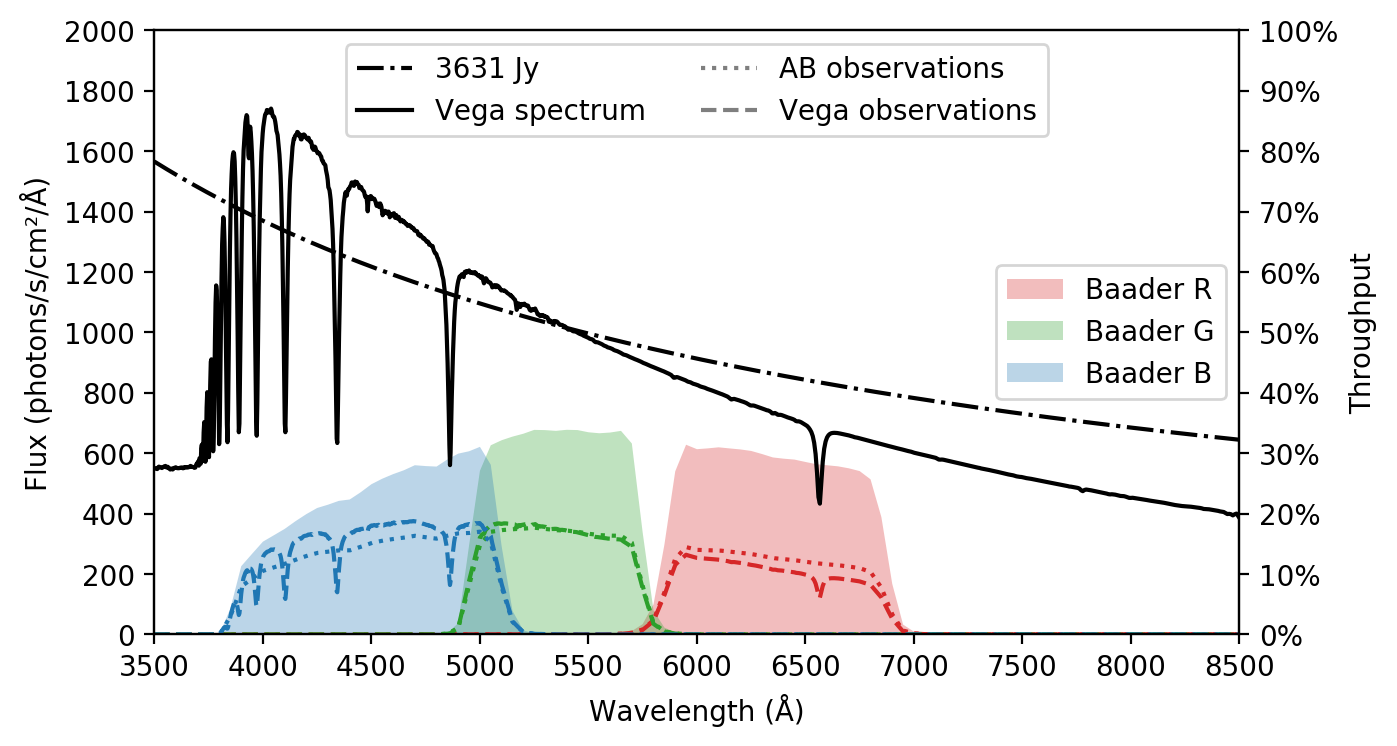
\includegraphics[width=\textwidth]{images/throughput/synphot.png}
    \end{center}
    \caption[Simulating photometric observations in the GOTO filters using pysynphot]{
        Simulating photometric observations in the GOTO filters using pysynphot. The filled coloured areas show the throughputs in the \textit{RGB} filters from \aref{fig:throughput}. The coloured dotted lines show the throughputs convolved with a flat \SI{3631}{\jansky} spectrum (dot-dashed black line), while the dashed lines show the throughputs convolved with the model Vega spectrum (solid black line). The same process was repeated for the \textit{L} filter (not shown for clarity).
    }\label{fig:pysynphot}
\end{figure}

\begin{table}[p]
    \begin{center}
        \begin{tabular}{c|cc|cc} %chktex 44
                   & \multicolumn{2}{c|}{AB system} & \multicolumn{2}{c}{Vega system}\\
            Filter & Signal    & Zeropoint & Signal    & Zeropoint\\
                   & (\elec/s) & (mag)     & (\elec/s) & (mag) \\
            \midrule
            Baader \textit{L} & \num{9.70e8} & 22.47 & \num{9.56e8} & 22.45 \\
            Baader \textit{R} & \num{2.96e8} & 21.18 & \num{2.51e8} & 21.00 \\
            Baader \textit{G} & \num{3.07e8} & 21.22 & \num{3.11e8} & 21.23 \\
            Baader \textit{B} & \num{3.98e8} & 21.50 & \num{4.38e8} & 21.60 \\
        \end{tabular}
    \end{center}
    \caption[Zeropoints in the AB and Vega systems calculated using pysynphot]{
        Zeropoints in the AB and Vega systems calculated using pysynphot.
    }\label{tab:pysynphot_zeropoints}
\end{table}

\clearpage

\end{colsection}

% ~~~~~~~~~~~~~~~~~~~~

\newpage
\subsection{Limiting magnitude}
\label{sec:lim_mag}
\begin{colsection}

Using the camera parameters determined in \aref{sec:detectors}, the throughput model created in \aref{sec:throughput} and the zeropoints calculated in \aref{sec:model_zeropoints} a complete photometric model of the GOTO telescopes can be created. One use of this is to predict the system limiting magnitude for a target signal-to-noise ratio.

% ---------
\subsubsection{Signal-to-noise}

The common sources of noise in CCDs are discussed in \aref{sec:noise}. Discounting the bias level and fixed-pattern noise, both properties of the camera which are easy to remove, the major sources of noise in an image will be the dark current and read-out noise. In addition, when taking on-sky images there will be a certain contamination level from background light. Accounting for these the total noise in the image is given by
%
\begin{equation}
    \sigma_\text{Total} = \sqrt{N + N_\text{BG} + D + R^2},
    \label{eq:total_noise}
\end{equation}
%
where $N$ is the electron signal from the source object, $N_\text{BG}$ is the additional signal from the background, $D$ is the dark current signal and $R$ is the read-out noise. Noise is usually quantified as a fraction of the target signal $N$, known as the signal-to-noise ratio:
%
\begin{equation}
    \text{SNR} = \frac{N}{\sigma_\text{Total}} = \frac{N}{\sqrt{N + N_\text{BG} + D + R^2}}.
    \label{eq:snr}
\end{equation}

For good science-quality observations a signal-to-noise value of 5 or more is required, also known as a $5\sigma$ detection (as the signal will be more than 5 times the noise).

\newpage

% ---------
\subsubsection{Background noise}

\begin{figure}[t]
    \begin{center}
        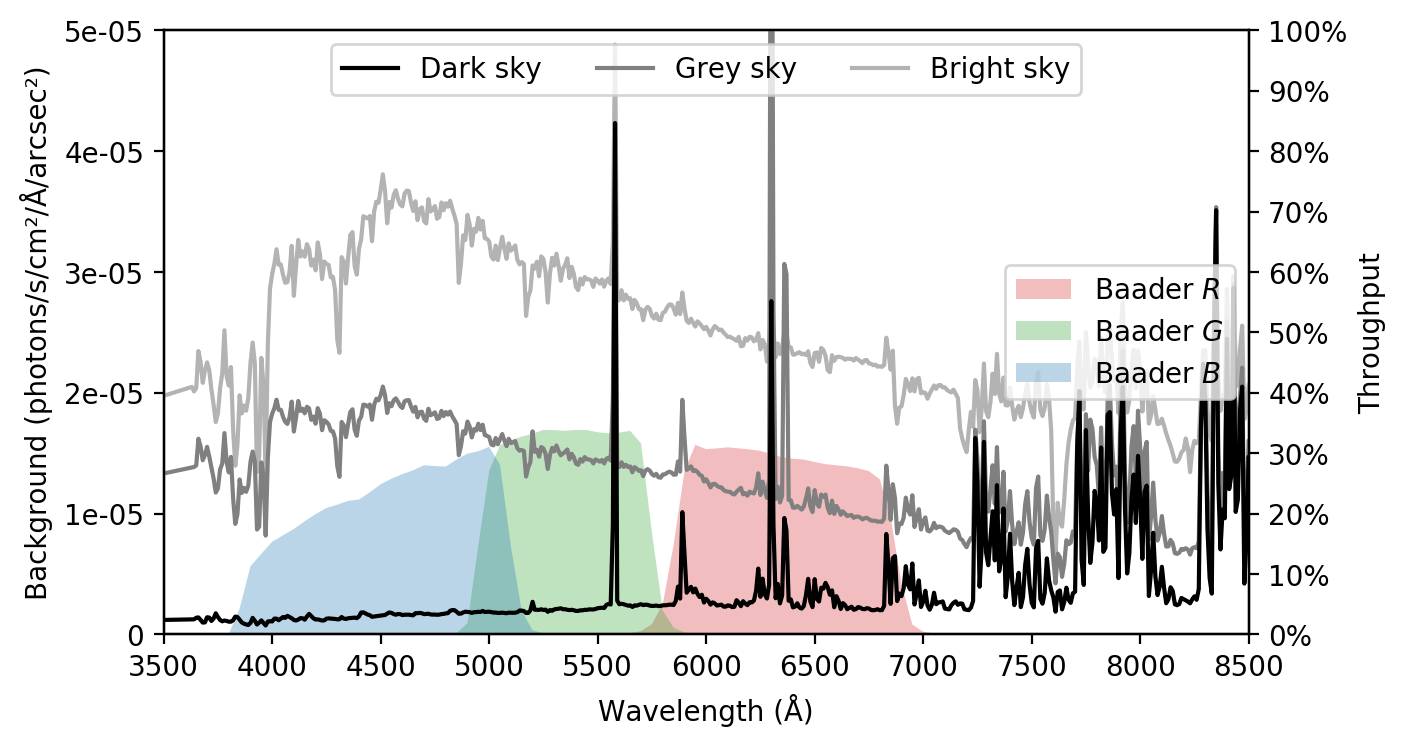
\includegraphics[width=\textwidth]{images/throughput/background.png}
    \end{center}
    \caption[Simulating sky background observations]{
        Simulating sky background observations in the GOTO filters using pysynphot. Compare to \aref{fig:pysynphot}.
    }\label{fig:background}
\end{figure}

The one value in \aref{eq:snr} that has not yet been considered is the background noise, $N_\text{BG}$. The brightness of the sky will change most noticeably as a function of the Moon phase, with a full Moon creating a background noise several magnitudes higher than during a new Moon or when the Moon is below the horizon. In order to model the background spectra were taken from \citet{sky_background}, which includes background spectra taken from 6 years of VLT observations using the FORS1 instrument\footnote{Spectra available at \href{http://www.eso.org/~fpatat/science/skybright}{\texttt{http://www.eso.org/\raisebox{0.5ex}{\texttildelow}fpatat/science/skybright}}}. Three sample spectra were selected to give a range of background signals: a ``Dark'' spectrum taken when the Moon was new and below the horizon, a ``Grey'' spectrum taken when the Moon was 60\% illuminated and a ``Bright'' spectrum when taken when the Moon was full. These spectra are shown in \aref{fig:background}.

The spectra were again convolved with the throughput model for each filter, and multiplied by the collecting area of the telescope, in order to get an expected signal in electrons per second. These were converted into instrumental magnitudes using \aref{eq:ins_mag} and then into true magnitudes using \aref{eq:zp} and the AB zeropoints given in \aref{tab:pysynphot_zeropoints}. The resulting background signals are given in \aref{tab:pysynphot_background}. Note that the background is given per square arcsecond; when calculating the background flux the signal must be multiplied by plate scale of the camera to get the signal per pixel (1.24 arcseconds/pixel for the MicroLine cameras).

\begin{table}[t]
    \begin{center}
        \begin{tabular}{c|ccc|ccc} %chktex 44
                   & \multicolumn{6}{c}{Background signal} \\
            Filter &
            \multicolumn{3}{c|}{(\elec/s/arcsec$^2$)} &
            \multicolumn{3}{c}{(mag/s/arcsec$^2$)} \\
                   & Dark & Grey & Bright & Dark & Grey & Bright \\
            \midrule
            Baader \textit{L} & 2.58 & 14.27 & 27.13 & 21.44 & 19.58 & 18.88 \\
            Baader \textit{R} & 1.18 &  4.37 &  8.20 & 20.99 & 19.58 & 18.89 \\
            Baader \textit{G} & 0.81 &  4.56 &  8.99 & 21.45 & 19.57 & 18.83 \\
            Baader \textit{B} & 0.52 &  5.74 & 10.65 & 22.20 & 19.60 & 18.93 \\
        \end{tabular}
    \end{center}
    \caption[Sky background signals calculated using pysynphot]{
        Sky background signals calculated using pysynphot for different Moon phases.
    }\label{tab:pysynphot_background}
\end{table}

% ---------
\subsubsection{Calculating limiting magnitudes}

The limiting magnitude of a telescope is defined by the signal which would be required to get over a particular SNR, for example $5\sigma$. \aref{eq:snr} therefore can be rearranged into a quadratic formula
%
\begin{equation}
    N_\text{lim}^2 - \text{SNR}^2 N_\text{lim} + \text{SNR}^2 (N_\text{BG} + D + R^2) = 0,
    \label{eq:snr2}
\end{equation}
%
and this can be solved to find $N_\text{lim}$.

It is important to remember that $N_\text{lim}$, $N_\text{BG}$ and $D$ are in electrons per second per pixel while $R$ is just in electrons per pixel (as the read-out noise is independent of the exposure time). Each therefore needs to be multiplied by the number of pixels the source is spread across, which will be the determined by the the size of the seeing disk. A given seeing $s$ in arcseconds is defined as the \glsfirst{fwhm} of the seeing disk in the image, and number of pixels the source will be spread across is
%
\begin{equation}
    n = \pi {\left(3 \frac{0.5s}{p}\right)}^2,
    \label{eq:seeing}
\end{equation}
%
where $p$ is the plate scale in arcseconds/pixel and the factor of three comes from taking the $3\sigma$ radius (note as the seeing is the FWHM it must be halved to get the radius).

Finally, the limiting magnitude in each filter and telescope can be calculated for a range of exposure times. These are plotted in \aref{fig:lim_mags} for dark and bright skies, for each GOTO filter and camera. Note it is almost impossible to distinguish between the lines for each camera, as the fractional difference between their dark and read out noise values are very small. The limiting magnitudes for a \SI{60}{\second} image, the typical exposure time for GOTO observations, are given in \aref{tab:lim_mags}.

\begin{figure}[t]
    \begin{center}
        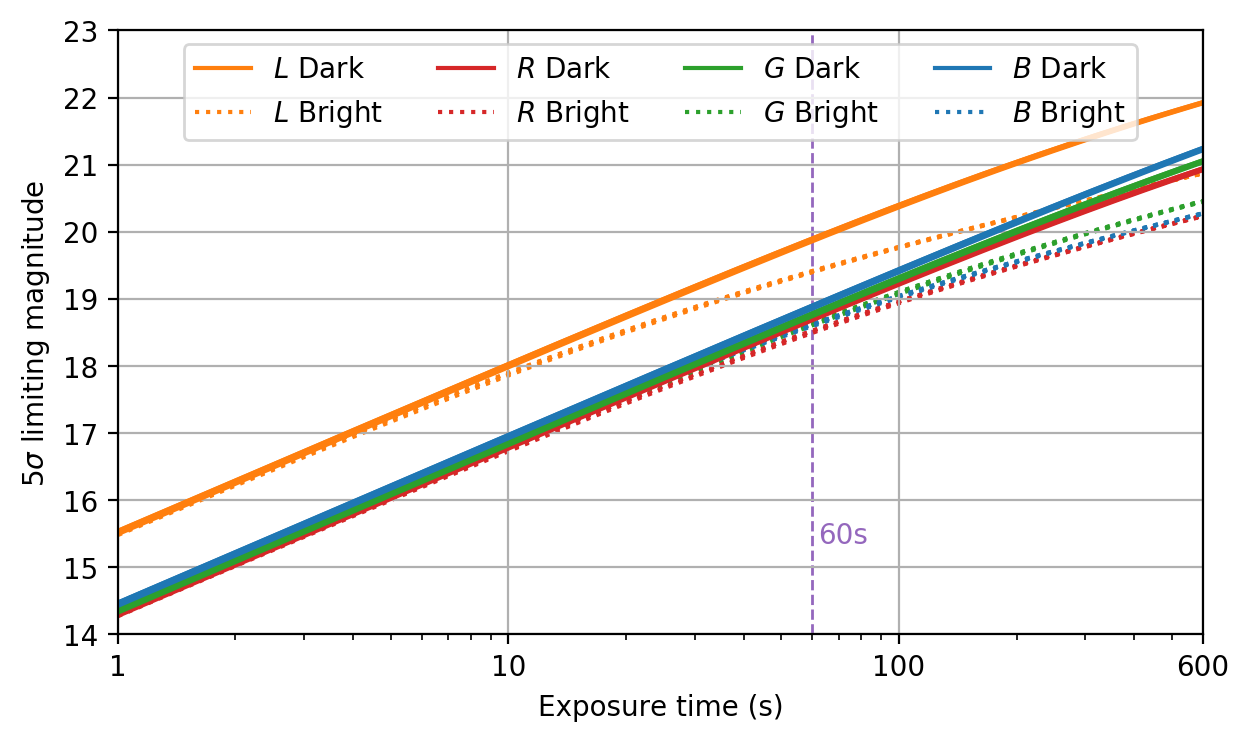
\includegraphics[width=\textwidth]{images/throughput/limiting_mag.png}
    \end{center}
    \caption[$5\sigma$ limiting magnitudes for GOTO]{
        $5\sigma$ limiting magnitudes for GOTO plotted as a function of exposure time, assuming an airmass of 1 and seeing of 1.5. Solid lines give the limiting magnitude during dark time, dotted lines during bright time. A vertical dashed line has been added at \SI{60}{\second}.
    }\label{fig:lim_mags}
\end{figure}

\begin{table}[t]
    \begin{center}
        \begin{tabular}{c|ccc} %chktex 44
                   & \multicolumn{3}{c}{Limiting magnitude} \\
            Filter & \multicolumn{3}{c}{(mag)} \\
                   & Dark & Grey & Bright \\
            \midrule
            Baader \textit{L} & 19.76 & 19.53 & 19.35 \\
            Baader \textit{R} & 18.51 & 18.43 & 18.35 \\
            Baader \textit{G} & 18.56 & 18.46 & 18.37 \\
            Baader \textit{B} & 18.85 & 18.72 & 18.62 \\
        \end{tabular}
    \end{center}
    \caption[$5\sigma$ limiting magnitudes for a \SI{60}{\second} exposure]{
        $5\sigma$ limiting magnitudes for a \SI{60}{\second} exposure in different filters and Moon phases.
    }\label{tab:lim_mags}
\end{table}

\end{colsection}

% ~~~~~~~~~~~~~~~~~~~~
\newpage
\subsection{Comparison to on-sky observations}
\label{sec:onsky_comparison}
\begin{colsection}

The GOTO prototype finally reached a stable 4-UT system in February 2019 (see \aref{sec:timeline}). In order to determine if it was performing to expectations the theoretical zeropoints and limiting magnitudes calculated in the previous sections can be compared to those found from real on-sky observations. Since GOTO is a very wide-field survey instrument there was no need to observe a particular standard star or field --- each frame contains thousands of individual sources that could be matched to a reference catalogue. In this case a set of sample observations were used: three \SI{60}{\second} exposures in all four filters (12 in total) of the Virgo Cluster, taken on the 16th of March 2019. These observations were taken during dark time and when the target was at a high altitude (airmass 1.08).

Each image was processed using the standard GOTO-photo pipeline (\todo{described in intro}), which calibrated the frames and extracted source counts using Source Extractor \citep{SE}. These counts were background-subtracted and converted into instrumental magnitudes using \aref{eq:ins_mag}, with $t=60$ and using the gain values for each camera calculated in \aref{sec:ptc}.

As GOTO uses the non-standard Baader filters (see \aref{sec:filters}) there are no exact catalogue magnitudes to compare to. The GOTO pipeline instead makes do with the best available catalogues: the Pan-STARRS PS1 catalogue \citep{Pan-STARRS} and APASS, the AAVSO Photometric All-Sky Survey \citep{APASS}. The \textit{L} and \textit{G} Baader filters are matched to Pan-STARRS \textit{g}, \textit{R} to Pan-STARRS \textit{r} and \textit{B} to APASS \textit{B}.

\begin{figure}[t]
    \begin{center}
        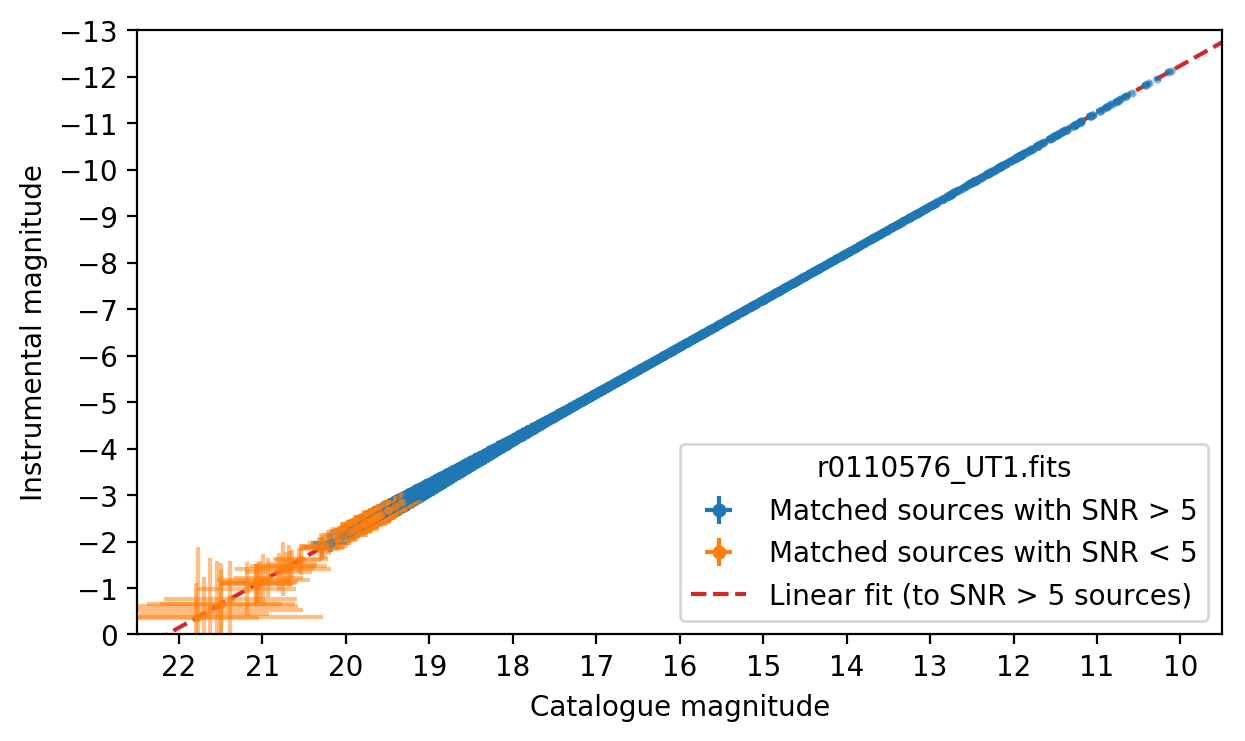
\includegraphics[width=\textwidth]{images/throughput/zeropoint_real.png}
    \end{center}
    \caption[Finding the observed zeropoint from a GOTO image]{
        Finding the observed zeropoint from a GOTO image.
    }\label{fig:zeropoint}
\end{figure}

In order to find the zeropoint for each image a linear function was fitted between the measured instrumental magnitudes of each source and the catalogue magnitude of the star it was matched against, with the y-intercept being equal to the zeropoint for that image. This is shown in \aref{fig:zeropoint} for one of the \textit{L}-band images. To exclude low-magnitude sources with large errors when fitting only sources with an SNR of 5$\sigma$ or above were included. This was repeated for every image, and the zeropoints for each are given in \aref{tab:zps_lms}.

To find the limiting magnitude the catalogue magnitude of each source was compared to the ratio of the source count and its measured noise. The $5\sigma$ limiting magnitude was taken as the mean magnitude of sources with a signal to noise ratio between 4.5 and 5.5. This method is plotted in \aref{fig:lim_mag}, and the limiting magnitude values and error values are also given in \aref{tab:zps_lms}.

\newpage

\begin{figure}[t]
    \begin{center}
        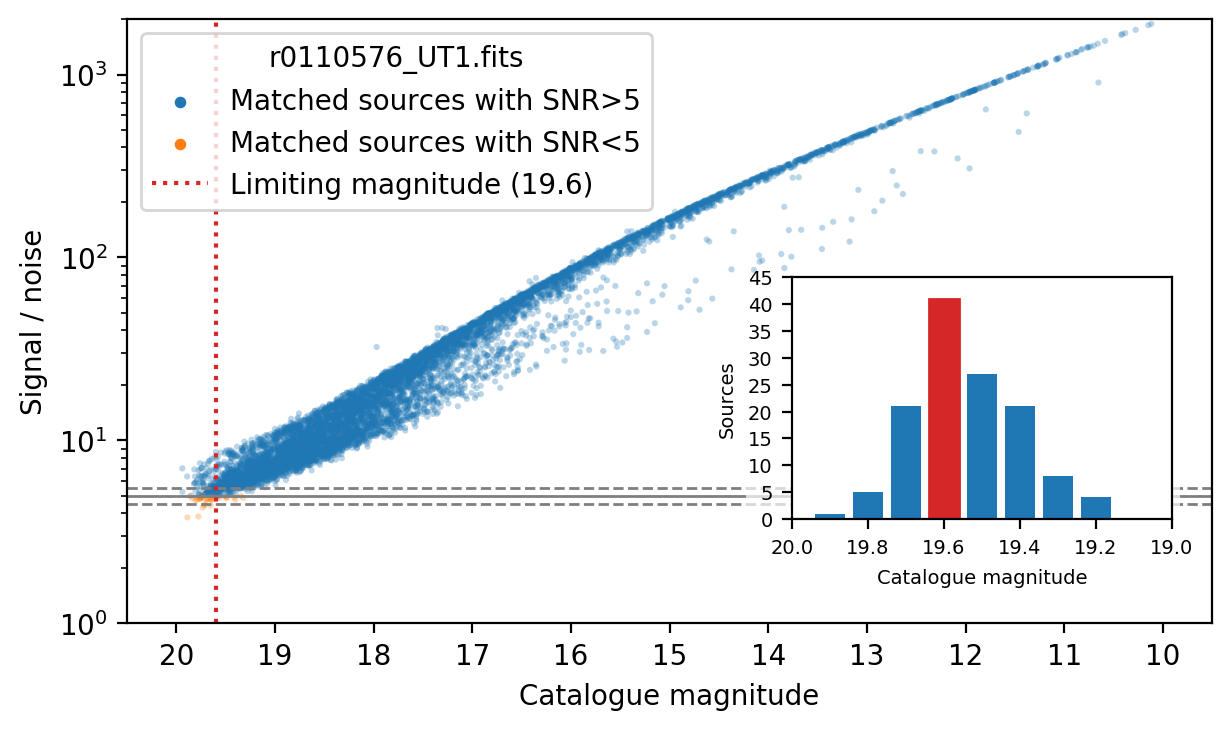
\includegraphics[width=\textwidth]{images/throughput/limiting_mag_real.png}
    \end{center}
    \caption[Finding the limiting magnitude from a GOTO image]{
        Finding the limiting magnitude from a GOTO image.
    }\label{fig:lim_mag}
\end{figure}

For each filter/unit telescope combination the best zeropoints and limiting magnitudes were selected from each set of three. These are given in \aref{tab:zps_comparison} and \aref{tab:lms_comparison}, and are compared to the theoretical AB magnitude zeropoints from \aref{tab:pysynphot_zeropoints} and the theoretical limiting magnitudes from \aref{tab:lim_mags}. In most cases the observed zeropoints and limiting magnitudes are very close to the theoretical values. Further images taken over more nights are needed to make any firm conclusions, but a few trends are clear. UT3 consistently has a better zeropoints than the others, which might be because its mirrors were serviced and returned only a month before the images were taken. Therefore the deficit in the observed zeropoints may be due to dust or imperfections that build up on the mirrors and reduce the throughput. It also seems that the throughput in the \textit{G} band has been underestimated, as the observations have higher zeropoints and better limiting magnitudes than predicted. This may be due to the bandwidth being wider than modelled, as any other change in throughput would also affect the other filters.

\newpage

\begin{table}[p]
    \begin{center}
        \begin{tabular}{cc|cc|cc|cc|cc} %chktex 44
             & &
            \multicolumn{2}{c|}{UT1} &
            \multicolumn{2}{c|}{UT2} &
            \multicolumn{2}{c|}{UT3} &
            \multicolumn{2}{c}{UT4}
            \\
             & &
            \multicolumn{2}{c|}{{\footnotesize(ML6094917)}} &
            \multicolumn{2}{c|}{{\footnotesize(ML0010316)}} &
            \multicolumn{2}{c|}{{\footnotesize(ML0420516)}} &
            \multicolumn{2}{c}{{\footnotesize(ML5644917)}}
            \\
            \multicolumn{2}{c|}{Filter} &
            ZP & LM & ZP & LM & ZP & LM & ZP & LM \\
            \midrule
            \textit{L} & 1 &
            22.32 & $19.6 \pm 0.2$ &
            22.31 & $19.7 \pm 0.3$ &
            22.40 & $19.7 \pm 0.2$ &
            22.32 & $19.6 \pm 0.1$
            \\
            & 2 &
            22.26 & $19.6 \pm 0.2$ &
            22.27 & $19.6 \pm 0.2$ &
            22.44 & $19.7 \pm 0.2$ &
            22.37 & $19.6 \pm 0.4$
            \\
            & 3 &
            22.39 & $19.6 \pm 0.2$ &
            22.42 & $19.8 \pm 0.4$ &
            22.45 & $19.7 \pm 0.2$ &
            22.40 & $19.6 \pm 0.3$
            \\
            \midrule
            \textit{R} & 1 &
            20.83 & $18.4 \pm 0.2$ &
            21.05 & $18.4 \pm 0.2$ &
            21.10 & $18.5 \pm 0.1$ &
            21.05 & $18.3 \pm 0.3$
            \\
            & 2 &
            20.84 & $18.4 \pm 0.2$ &
            21.11 & $18.5 \pm 0.3$ &
            21.13 & $18.4 \pm 0.2$ &
            21.06 & $18.3 \pm 0.3$
            \\
            & 3 &
            20.91 & $18.3 \pm 0.2$ &
            21.01 & $18.5 \pm 0.4$ &
            21.04 & $18.4 \pm 0.2$ &
            20.94 & $18.3 \pm 0.1$
            \\
            \midrule
            \textit{G} & 1 &
            21.20 & $18.7 \pm 0.2$ &
            21.39 & $18.8 \pm 0.3$ &
            21.40 & $18.8 \pm 0.2$ &
            21.27 & $18.7 \pm 0.3$
            \\
            & 2 &
            21.16 & $18.7 \pm 0.2$ &
            21.43 & $18.8 \pm 0.3$ &
            21.46 & $18.8 \pm 0.2$ &
            21.36 & $18.7 \pm 0.3$
            \\
            & 3 &
            21.26 & $18.7 \pm 0.2$ &
            21.44 & $18.8 \pm 0.2$ &
            21.45 & $18.8 \pm 0.1$ &
            21.32 & $18.6 \pm 0.2$
            \\
            \midrule
            \textit{B} & 1 &
            21.22 & $19.0 \pm 0.2$ &
            21.35 & $19.1 \pm 0.3$ &
            21.43 & $19.1 \pm 0.2$ &
            21.27 & $19.1 \pm 0.4$
            \\
            & 2 &
            21.22 & $19.0 \pm 0.2$ &
            21.32 & $19.0 \pm 0.4$ &
            21.44 & $19.1 \pm 0.2$ &
            21.22 & $19.1 \pm 0.3$
            \\
            & 3 &
            21.20 & $19.1 \pm 0.2$ &
            21.35 & $19.0 \pm 0.4$ &
            21.44 & $19.1 \pm 0.2$ &
            21.26 & $19.1 \pm 0.3$
            \\
        \end{tabular}
    \end{center}
    \caption[Observed zeropoints and limiting magnitudes]{
        Observed zeropoints and limiting magnitudes from three \SI{60}{\second} exposures taken in each filter. The camera serial numbers can be matched to \aref{tab:cameras}.
    }\label{tab:zps_lms}
\end{table}

\begin{table}[p]
    \begin{center}
        \begin{tabular}{c|c|cccc|cccc} %chktex 44
             &
            Theoretical &
            \multicolumn{4}{c|}{Best observed zeropoint} &
            \multicolumn{4}{c}{Difference (obs-theory)}
            \\
            Filter & zeropoint & UT1 & UT2 & UT3 & UT4 & UT1 & UT2 & UT3 & UT4 \\
            \midrule
            \textit{L} & 22.47 & 22.39 & 22.42 & 22.45 & 22.40 & -0.08 & -0.05 & -0.02 & -0.07 \\
            \textit{R} & 21.18 & 20.91 & 21.11 & 21.13 & 21.06 & -0.27 & -0.07 & -0.05 & -0.12 \\
            \textit{G} & 21.22 & 21.26 & 21.44 & 21.46 & 21.36 & +0.04 & +0.22 & +0.24 & +0.14 \\
            \textit{B} & 21.50 & 21.22 & 21.35 & 21.44 & 21.27 & -0.28 & -0.15 & -0.06 & -0.23 \\
        \end{tabular}
    \end{center}
    \caption[Comparison between theoretical and observed zeropoints]{
        Comparison between the best observed zeropoints and the theoretical AB magnitude zeropoints from \aref{tab:pysynphot_zeropoints}.
    }\label{tab:zps_comparison}
\end{table}

\begin{table}[p]
    \begin{center}
        \begin{tabular}{c|c|cccc} %chktex 44
             &
            Theoretical &
            \multicolumn{4}{c}{Best observed limiting magnitude}
            \\
            Filter & limiting magnitude & UT1 & UT2 & UT3 & UT4 \\
            \midrule
            \textit{L} & 19.76 & $19.6 \pm 0.2$ & $19.8 \pm 0.4$ & $19.7 \pm 0.2$ & $19.6 \pm 0.3$ \\
            \textit{R} & 18.51 & $18.4 \pm 0.2$ & $18.5 \pm 0.3$ & $18.5 \pm 0.1$ & $18.3 \pm 0.3$ \\
            \textit{G} & 18.56 & $18.7 \pm 0.2$ & $19.8 \pm 0.3$ & $18.8 \pm 0.2$ & $18.7 \pm 0.3$ \\
            \textit{B} & 18.85 & $19.1 \pm 0.2$ & $19.1 \pm 0.3$ & $19.1 \pm 0.2$ & $19.1 \pm 0.3$ \\
        \end{tabular}
    \end{center}
    \caption[Comparison between theoretical and observed limiting magnitudes]{
        Comparison between the best observed limiting magnitudes and the theoretical dark-time limiting magnitudes from \aref{tab:lim_mags}.
    }\label{tab:lms_comparison}
\end{table}

\clearpage

\end{colsection}

% ~~~~~~~~~~~~~~~~~~~~

\end{colsection}

% ########################################
